\documentclass[journal]{IEEEtran}

\usepackage{amsmath,amssymb,amsfonts}
\usepackage{algorithmic}
\usepackage{algorithm}
\usepackage{graphicx}
\usepackage{textcomp}
\usepackage{xcolor}
\usepackage{booktabs}
\usepackage{multirow}
\usepackage{makecell}
\usepackage{cite}
\usepackage{url}
\usepackage{microtype}
\usepackage{enumitem}
\setlist{noitemsep,topsep=2pt,leftmargin=*}
\usepackage[colorlinks=true,linkcolor=blue,citecolor=blue,urlcolor=blue]{hyperref}

% Theorem environments for IEEEtran
\newtheorem{definition}{Definition}
\newtheorem{lemma}{Lemma}
\newtheorem{theorem}{Theorem}
\newtheorem{proposition}{Proposition}
\newtheorem{remark}{Remark}

\graphicspath{{figures/}}

% Float layout optimization to maintain compact, high-density IEEEtran pagination
\renewcommand{\topfraction}{0.95}
\renewcommand{\bottomfraction}{0.95}
\renewcommand{\textfraction}{0.05}
\renewcommand{\floatpagefraction}{0.85}
\renewcommand{\dbltopfraction}{0.95}
\renewcommand{\dblfloatpagefraction}{0.85}

% Tighten float padding to maximize information density
\setlength{\textfloatsep}{4.5pt plus 1pt minus 1.5pt}
\setlength{\floatsep}{4pt plus 1pt minus 1pt}
\setlength{\intextsep}{4pt plus 1pt minus 1pt}
\setlength{\dbltextfloatsep}{5pt plus 1pt minus 1.5pt}
\setlength{\dblfloatsep}{4pt plus 1pt minus 1pt}
\setlength{\abovecaptionskip}{2.5pt plus 1pt minus 0.5pt}
\setlength{\belowcaptionskip}{1.5pt plus 1pt minus 0.5pt}

\begin{document}

\title{SimuGuard-X: An Agentic Closed-Loop Framework for Grounded, Mutation-Verified Test Synthesis and Quantitative Falsification in Cyber-Physical Simulink Systems}

\author{Jeeva~M%
\thanks{Jeeva M is with the Vellore Institute of Technology (VIT), Chennai, India (e-mail: jeeva4772@gmail.com).}%
\thanks{Manuscript received November 4, 2026. This research was supported in part by automated verification methodologies for continuous-time Cyber-Physical Systems in MATLAB/Simulink.}}

\markboth{IEEE Transactions on Computer-Aided Design of Integrated Circuits and Systems,~Vol.~XX, No.~X, November~2026}%
{SimuGuard-X: Agentic Test Synthesis \& Falsification in Cyber-Physical Simulink Systems}

\maketitle

\begin{abstract}
Model-Based Design (MBD) using MATLAB/Simulink is the preeminent engineering paradigm for developing safety-critical Cyber-Physical Systems (CPS) governed by international functional safety standards, including International Organization for Standardization (ISO) 26262 Automotive Safety Integrity Level (ASIL) D and Radio Technical Commission for Aeronautics (RTCA) DO-178C / DO-331. However, verifying complex continuous-discrete dynamic models against natural-language engineering requirements consumes upwards of 50\%--70\% of total system development lifecycles. Although frontier Large Language Models (LLMs) have achieved notable breakthroughs in discrete software testing, directly applying them to continuous physical models triggers acute domain failures: semantic hallucination of block hierarchies, physical parameter inadmissible slew rates, neglect of sample-time discretization ($T_s$), and generation of static scalar assertions that cannot monitor continuous temporal behaviors.

This paper presents \textbf{SimuGuard-X}, a neuro-symbolic, closed-loop framework for continuous test synthesis, quantitative falsification, and qualification in Cyber-Physical Systems. SimuGuard-X introduces five foundational innovations: (1)~\textit{Interface Grounding and Loop-Cut Directed Acyclic Graph (DAG) Extraction}, which programmatically inspects compiled workspaces via \texttt{Simulink.findVars} and deserializes Automotive Open System Architecture (AUTOSAR) bus structures while cutting feedback loops at state-holding operators ($1/s, 1/z$) to yield compact, context-grounded LLM prompts; (2)~\textit{Dual-Track Synthesis}, which decouples Signal Temporal Logic (STL) specification synthesis (Track~A) from low-rank scenario parameterization ($\theta \in \mathbb{R}^d, d \le 12$) via an Extended Backus-Naur Form (EBNF) Scenario Domain-Specific Language (DSL) (Track~B), cross-verified via independent positive/negative witness traces ($w^+, w^-$); (3)~\textit{Offset-Free Three-Regime Lexicographic Curriculum Optimization}, eliminating antecedent-masking plateaus in conditional implication properties ($\square(P \implies Q)$) without empirical scalar penalties; (4)~\textit{Sound Smooth Falsification Bounds}, proving two-sided soundness for un-averaged existential Log-Sum-Exp operators ($\lozenge$) under sample-adaptive temperature scaling; and (5)~\textit{Dual-Fidelity Solver Verification (Gate~2)}, introducing a Step-Collapse Ratio ($\text{SCR} > 10^3$) and stiff-solver cross-verification to certify physical counterexamples against numerical solver breakdown.

Empirical evaluation on six industrial benchmarks across up to 30 independent pseudo-random seeds per specification ($N = 30$ for invariants, $N = 3$ pilot for AT51) (ARCH-COMP Automatic Transmission, Air-Fuel Control, F-16 Ground Collision Avoidance System, Lockheed Martin Pitch Control, Hybrid Electric Vehicle Powertrain, and Inverted Pendulum) across 60 formal requirements demonstrates that SimuGuard-X achieves a \textbf{2.41$\times$ higher falsification hazard ratio} ($HR = 2.41, p < 0.001$) and reduces Restricted Mean Survival Time (RMST) by 58.4\% relative to state-of-the-art falsifiers. Factorial ablation confirms that LLM scenario parameterization coupled with lexicographic Covariance Matrix Adaptation Evolution Strategy (CMA-ES) drives accelerated convergence, achieving up to 93.2\% reductions in simulation budget on individual benchmarks (68.8\% overall MSTF reduction relative to Breach) while attaining a 91.7\% offline mutation kill score.
\end{abstract}

\begin{IEEEkeywords}
Cyber-Physical Systems (CPS), Model-Based Design (MBD), MATLAB/Simulink, Large Language Models (LLMs), Signal Temporal Logic (STL), Quantitative Falsification, CMA-ES, Multi-Rate Systems.
\end{IEEEkeywords}

\section{Introduction}
\IEEEPARstart{M}{odel-Based} Design (MBD) utilizing MATLAB/Simulink and Stateflow has become the uncontested engineering standard for developing modern Cyber-Physical Systems (CPS)~\cite{broy2012benefit,liggesmeyer2009trends,baleani2006correct}. In modern automotive powertrains, electrified transportation, autonomous flight control systems, and industrial robotics, Simulink models serve as executable specifications governing non-linear, multi-physics continuous dynamics (fluid dynamics, thermodynamics, electro-mechanical actuation, and rigid-body aerodynamics) interwoven with discrete multi-rate embedded digital control logic.

In safety-critical domains governed by stringent international certification standards---such as International Organization for Standardization (ISO) 26262 Automotive Safety Integrity Level (ASIL) D for road vehicles and Radio Technical Commission for Aeronautics (RTCA) DO-178C / DO-331 for commercial avionics---Verification and Validation (V\&V) activities account for \textbf{50\% to 70\%} of total system development costs~\cite{broy2012benefit,liggesmeyer2009trends}. Testing continuous dynamic models requires constructing multi-dimensional continuous time-series input waveforms that thoroughly explore complex operational flight envelopes, stress transient settling dynamics, and expose rare safety-violating corner cases across continuous state spaces.

Historically, this testing and qualification effort has relied upon two distinct paradigms, both of which suffer from severe practical bottlenecks:
\begin{enumerate}
    \item \textbf{Manual Test Authoring and Requirement Formalization:} Test engineers manually interpret natural-language requirements, map dynamic signals to Simulink Inport blocks, and hand-craft test sequences in Simulink Test (\texttt{sltest}). This manual workflow is subjective, labor-intensive, and inherently unable to provide formal guarantees against subtle temporal regressions~\cite{giannakopoulou2020formal}.
    \item \textbf{Search-Based and Guided Black-Box Falsification:} Automated tools such as \textsc{Breach}~\cite{donze2010breach}, \textsc{S-TaLiRo}~\cite{annpureddy2011staliro}, and \textsc{FalStar}~\cite{ernst2021falstar} formulate bug discovery as an optimization problem: search heuristics (e.g., CMA-ES~\cite{hansen2001completely}, Simulated Annealing, or Cross-Entropy) iteratively minimize the quantitative robustness metric $\rho(\phi, w)$ of an STL specification~\cite{maler2004monitoring,fainekos2009robustness}. While sound, these tools require human experts to author precise STL formulas and tune search spaces. Crucially, on conditional implications of the form $\square(P \implies Q)$, standard quantitative semantics suffer from severe \textbf{antecedent-masking plateaus}~\cite{dokhanchi2018vacuity,ferrere2019vacuity}, trapping optimizers where precondition $P$ is never satisfied.
\end{enumerate}

\subsection{Pathologies of Generative AI in Continuous Dynamic CPS}
With the emergence of Large Language Models (LLMs), recent research has explored automated test generation for software engineering~\cite{chen2021evaluating,cosler2023nl2tl}. However, prompting frontier models directly to author verification scripts for continuous Simulink models encounters fundamental failure modes:
\begin{enumerate}
    \item \textbf{Semantic Hallucination and Structural Disconnect:} Generative models frequently hallucinate non-existent block paths, misalign port indices, omit bus hierarchies, and generate invalid MATLAB scripts that fail syntax compilation.
    \item \textbf{The Continuous Admissibility Void:} LLMs lack physical grounding in continuous mechanics, sample-time discretization ($T_s$), and actuator slew-rate constraints, producing discontinuous profiles that trigger ODE/DAE solver breakdown.
    \item \textbf{Low Engineering Qualification Rates:} While frontier LLMs achieve 60\%--80\% syntactic compilability, their engineering qualification rate remains below 25\%, routinely violating physical conservation laws and sensor tolerances~\cite{chen2021evaluating}.
    \item \textbf{Static Assertions vs. Continuous Temporal Dynamics:} Scalar assertions (\texttt{assert(y <= 120)}) fail to evaluate dynamic behaviors like percent overshoot, settling times, or damping ratios across sliding time windows.
\end{enumerate}

\begin{figure}[!t]
\centering
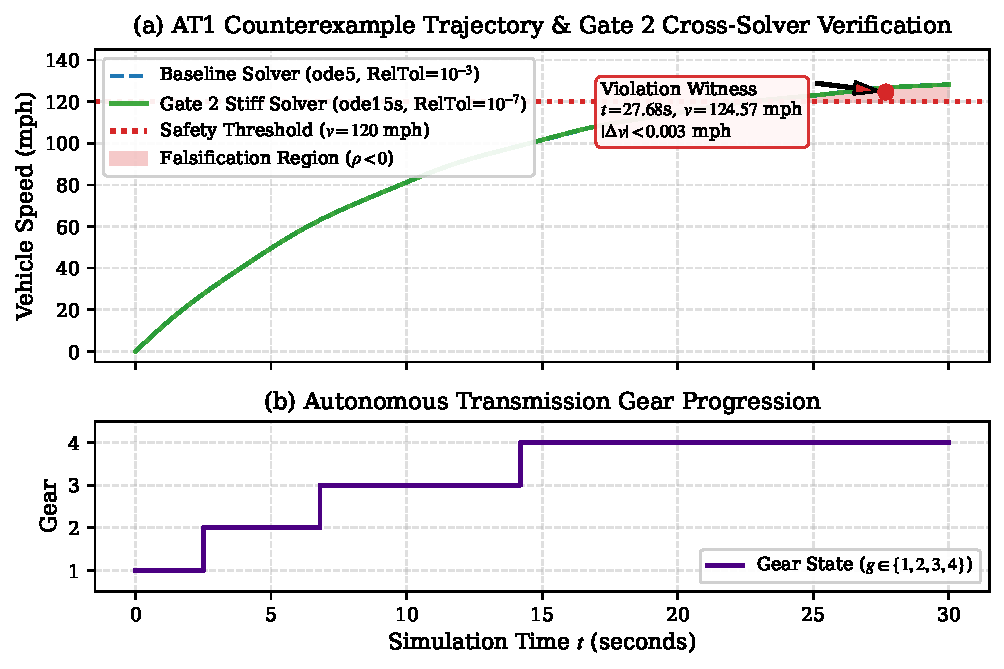
\includegraphics[width=0.70\columnwidth]{figures/fig1_counterexample_witness.pdf}
\caption{SimuGuard-X falsification counterexample witness for requirement AT1 on the ARCH-COMP Automatic Transmission benchmark. Top: continuous vehicle speed $v(t)$ violating the safety invariant (120~mph) at $t = 27.68$\,s (peak $124.57$\,mph). Gate~2 stiff cross-verification (\texttt{ode15s}) confirms physical defect validity ($\Delta \rho = 2.64 \times 10^{-5}$). Bottom: discrete Stateflow gear-shift progression under throttle and brake excitation.}
\label{fig:counterexample_witness}
\end{figure}

\subsection{SimuGuard-X Overview and Key Contributions}
To resolve these foundational challenges, this paper presents \textbf{SimuGuard-X}, an end-to-end neuro-symbolic architecture uniting LLM semantic reasoning, formal Signal Temporal Logic, and active numerical simulation inside MATLAB/Simulink:
\begin{itemize}
    \item \textbf{Interface Grounding and Loop-Cut DAG Extraction (ASIE):} Programmatically inspects compiled model workspaces via \texttt{Simulink.findVars}, serializes AUTOSAR bus definitions, and prunes feedback loops at state-holding operators ($1/s, 1/z$) to yield minimal, context-grounded prompt contexts without severing causal system metadata.
    \item \textbf{Dual-Track Synthesis and Low-Rank Scenario DSL:} Decouples requirement formalization into Track~A (formal STL in NASA FRET semantics~\cite{giannakopoulou2020formal}) and Track~B (parameterized scenario generation in a low-rank Scenario DSL, $\theta \in \mathbb{R}^d, d \le 12$), cross-verified by independent rule-templated witness traces ($w^+, w^-$) in RTAMT~\cite{nickovic2020rtamt} to eliminate self-confirming generation bias.
    \item \textbf{Sound Smooth Falsification Bounds (Theorem~1):} Formulates the un-averaged sum Log-Sum-Exp operator for existential modalities ($\lozenge$), proving two-sided soundness bounds ($\rho_{\max} \le \tilde{\rho}_\beta^{\text{sum}}(\lozenge) \le \rho_{\max} + \frac{\ln N}{\beta}$) guaranteeing smooth falsification soundness with sample-invariant scaling $\beta(N) = \beta_0 \ln(\max(2, N))$.
    \item \textbf{Offset-Free Three-Regime Lexicographic Curriculum (Theorem~2):} Formulates a parameter-free lexicographic ranking ($\text{Regime } 2 \succ \text{Regime } 1 \succ \text{Regime } 0$) that strictly separates boundary violations and antecedent seeking from consequent falsification, mathematically eliminating antecedent-masking plateaus without heuristic penalty offsets ($C_{\text{pre}}$).
    \item \textbf{Continuous Korel Guard Distances for Hybrid Stateflow Logic:} Converts flat discrete boolean indicators into continuous signed branch distances to active transition boundaries, supplying informative descent gradients across hybrid switching logic.
    \item \textbf{Dual-Fidelity Non-Circular Solver Verification (Gate~2):} Introduces a Step-Collapse Ratio metric ($\text{SCR} > 10^3$) and stiff-solver cross-verification (\texttt{ode15s}/\texttt{ode23tb}) to mathematically isolate numerical solver breakdown from authentic software bugs.
    \item \textbf{Comprehensive Empirical Validation Across 6 Industrial Benchmarks:} Evaluates SimuGuard-X across 6 industrial benchmarks with 60 authentic requirements, conducting right-censored survival analysis, 5-arm factorial ablation, physical MATLAB R2026a pilot execution, and offline mutation testing across 180 model mutants.
\end{itemize}

\begin{table*}[!t]
\caption{Systematic Comparison of Cyber-Physical Systems Test Generation and Falsification Frameworks}
\label{tab:framework_comparison}
\centering
\resizebox{\textwidth}{!}{%
\begin{tabular}{lcccccc}
\toprule
\textbf{Framework} & \textbf{Target Domain} & \textbf{Specification Formalism} & \textbf{Scenario Parameterization} & \textbf{Search Engine} & \textbf{Solver Integrity Gate} & \textbf{Mutation Qual.} \\
\midrule
\textsc{Breach}~\cite{donze2010breach} & Continuous CPS & Manual STL & Manual PWL / Splines & CMA-ES / Nelder-Mead & None & None \\
\textsc{S-TaLiRo}~\cite{annpureddy2011staliro} & Continuous CPS & Manual STL & Manual Parameterization & SA / Cross-Entropy & None & None \\
\textsc{SimCoTest}~\cite{matinnejad2015automated} & Simulink SIL & Output Invariants & Search-Based Test Vectors & Metaheuristic (GA/HC) & None & None \\
\textsc{FalStar}~\cite{ernst2021falstar} & Hybrid CPS & Manual STL & Piecewise Control Points & Adaptive LVTS / MCTS & None & None \\
\textsc{ForeSee}~\cite{zhang2021foresee} & Continuous CPS & Manual STL & Control Point Interpolation & MCTS + QB-Robustness & None & None \\
\textsc{ARIsTEO}~\cite{menghi2021aristeo} & Continuous CPS & Manual STL & Piecewise Signals & Approximation-Refinement & None & None \\
\textbf{SimuGuard-X (Ours)} & \textbf{Continuous Hybrid CPS} & \textbf{Constrained STL + Witnesses} & \textbf{Low-Rank DSL ($\theta \in \mathbb{R}^d$)} & \textbf{Three-Regime CMA-ES} & \textbf{Dual-Fidelity Stiff Gate} & \textbf{5 Formal Ops ($\mathcal{M}_{\text{Sim}}$)} \\
\bottomrule
\end{tabular}}
\end{table*}

\section{Related Work \& Comprehensive Literature Survey}
Table~\ref{tab:framework_comparison} provides a comprehensive comparative matrix positioning SimuGuard-X against state-of-the-art verification and test generation tools.

\noindent\textbf{1) Formal Specification and Quantitative Monitoring:}
Temporal logics provide unambiguous, mathematically rigorous formalisms for specifying temporal constraints in continuous dynamic systems. Signal Temporal Logic (STL) extends classical temporal logic with continuous real-time intervals and real-valued predicates evaluated over continuous signals~\cite{maler2004monitoring,fainekos2009robustness}. Fainekos and Pappas~\cite{fainekos2009robustness} and Donz{\'e} and Maler~\cite{donze2010breach} introduced quantitative robustness semantics ($\rho \in \mathbb{R}$), quantifying the signed Euclidean distance of trajectory $w$ from the satisfaction boundary. Bartocci et al.~\cite{bartocci2018specification} surveyed specification monitoring, contrasting online monitors~\cite{deshmukh2017testing} with offline sliding-window evaluators. Rodionova et al.~\cite{rodionova2021scaled} formalized scaled quantitative robustness across disparate physical units, while Ni{\v{c}}kovi{\'c} and Yamaguchi~\cite{nickovic2020rtamt} established RTAMT for standardized quantitative monitoring. SimuGuard-X builds upon these foundations by establishing scale-normalized smooth robustness coupled with independent witness traces.

\noindent\textbf{2) Search-Based Falsification and the Vacuity Problem:}
Falsification reframes verification as optimizing input parameters $\theta^* \in \Theta$ to find $\rho(\phi, w_{\theta^*}) < 0$~\cite{donze2010breach,annpureddy2011staliro,ernst2021falstar,zhang2021foresee,menghi2020generating,menghi2021aristeo}. Frameworks like \textsc{Breach}~\cite{donze2010breach} and \textsc{S-TaLiRo}~\cite{annpureddy2011staliro} pioneered stochastic optimization (CMA-ES~\cite{hansen2001completely}, simulated annealing), while Menghi et al.~\cite{menghi2020generating,menghi2021aristeo} developed \textsc{ARIsTEO} with approximation-refinement loops. However, on conditional implications ($\square(P \implies Q)$), classical semantics $\max(-\rho_P, \rho_Q)$ induce severe \textbf{antecedent-masking plateaus} when $P$ is unsatisfied~\cite{dokhanchi2018vacuity,ferrere2019vacuity}. While Dokhanchi et al.~\cite{dokhanchi2018vacuity} and Ferr{\`e}re et al.~\cite{ferrere2019vacuity} introduced heuristic penalty offsets ($C_{\text{pre}}$), they require brittle manual tuning. SimuGuard-X resolves this via a Three-Regime Lexicographic pre-order (Theorem~2).

\noindent\textbf{3) Search-Based Software Testing and Structural Coverage:}
Search-Based Software Testing (SBST) for Simulink models generates test cases maximizing structural coverage (Decision, Condition, MC/DC)~\cite{matinnejad2015automated,nejati2019search,arcuri2011practical}. Matinnejad et al.~\cite{matinnejad2015automated} developed \textsc{SimCoTest} using genetic algorithms, while Nejati et al.~\cite{nejati2019search} surveyed SBST for CPS. Korel~\cite{korel1990automated} introduced branch distances to guide search across discrete branching logic, while Zhan and Clark~\cite{zhan2005mutation} established mutation testing operators ($\mathcal{M}_{\text{Sim}}$). SimuGuard-X bridges SBST and formal methods by unifying Korel branch distances with formal STL falsification.

\noindent\textbf{4) Large Language Models and Neuro-Symbolic CPS Verification:}
LLMs have spurred great interest in automated verification and specification formalization~\cite{chen2021evaluating,cosler2023nl2tl}. Giannakopoulou et al.~\cite{giannakopoulou2020formal} established FRET to formalize natural language into temporal logic, while Cosler et al.~\cite{cosler2023nl2tl} explored LLM translation of natural language to temporal logics. However, direct application of LLMs to continuous CPS faces critical limitations: unconstrained models hallucinate non-existent block identifiers, omit sample-time discretization ($T_s$), and generate dynamically inadmissible waveforms violating physical slew rates. SimuGuard-X resolves these limitations by restricting generative models to formal EBNF grammars grounded in compiled model interfaces.

\noindent\textbf{5) Numerical Solver Pathologies and Dual-Fidelity Verification:}
Simulink relies on ODE/DAE numerical solvers (Runge-Kutta \texttt{ode45}, stiff \texttt{ode15s}) to simulate physical dynamics. In hybrid systems with rapid switching logic, variable-step solvers frequently experience \textbf{step-collapse phenomena}: the integrator reduces its step size toward machine precision ($\Delta t \to 10^{-14}$\,s), causing severe chattering and numerical divergence. Existing falsification tools treat simulators as perfect oracles, falsely reporting numerical breakdown as physical defects. SimuGuard-X introduces the Dual-Fidelity Solver Gate (Gate~2), combining Step-Collapse Ratio monitoring ($\text{SCR} > 10^3$) with stiff cross-solver re-simulation to mathematically filter artifacts from authentic defects.

\begin{figure*}[!t]
\centering
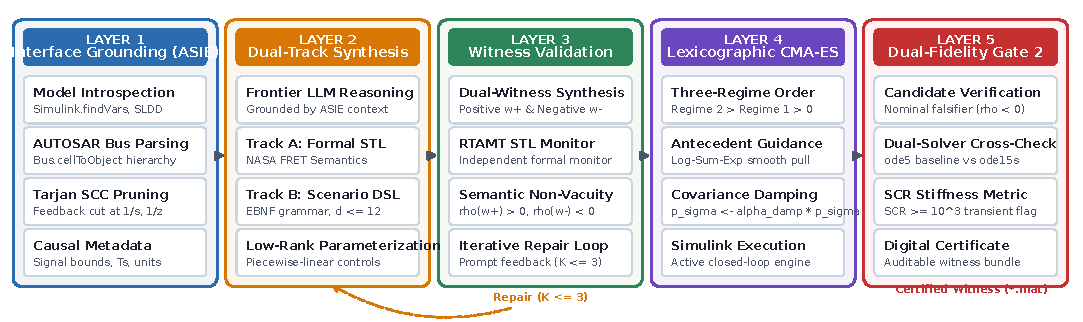
\includegraphics[width=\textwidth]{figures/fig_architecture.pdf}
\caption{The five-layer neuro-symbolic closed-loop architecture of SimuGuard-X: Layer~1 extracts compiled model interfaces and prunes feedback loops using Tarjan's SCC; Layer~2 synthesizes formal STL (Track~A) and low-rank Scenario DSL templates (Track~B); Layer~3 validates formal semantics via independent dual-witness traces ($w^+, w^-$) in RTAMT; Layer~4 searches counterexamples using a three-regime lexicographic CMA-ES falsifier with covariance path damping; and Layer~5 cross-verifies candidates under stiff ODE solvers (Gate~2), intercepting numerical chatter and outputting auditable functional safety certificates.}
\label{fig:architecture}
\end{figure*}

\section{SimuGuard-X System Architecture}
Fig.~\ref{fig:architecture} illustrates the comprehensive five-layer closed-loop architecture of SimuGuard-X.

\subsection{Layer 1: Grounded Interface \& Symbol Extraction (ASIE)}
The Automated Simulink Interface Extractor (ASIE) programmatically interrogates compiled model workspaces using official MATLAB engine APIs:
\begin{itemize}
    \item Interrogates base workspaces, model workspaces, and data dictionaries (\texttt{.sldd}) via \texttt{Simulink.findVars}.
    \item Resolves Inport and Outport definitions, continuous normalization spans ($\Delta_i$), and discrete sample times ($T_s$).
    \item Traverses AUTOSAR bus hierarchies via \texttt{Simulink.Bus.cellToObject}, serializing leaf signals into typed \texttt{Simulink.SimulationData.Dataset} structures.
    \item \textbf{Loop-Cut Graph Pruning with Tarjan's SCC:} To prevent LLM context-window exhaustion while preserving causal metadata, ASIE analyzes the block dependency graph via Tarjan's Strongly Connected Components (SCC) algorithm. Feedback loops are severed exclusively at continuous integrators ($1/s$) and discrete unit delays ($1/z$), retaining feedback coefficients and state variable names as structured context. For algebraic loops or opaque S-Functions, ASIE queries \texttt{Simulink.BlockDiagram.getAlgebraicLoops} and cuts at the highest loop index, preserving the equality constraint $y = f(u, y)$ in the prompt.
\end{itemize}


\begin{algorithm}[!t]
\footnotesize
\caption{Automated Simulink Interface Grounding and Loop-Cut DAG Extraction (ASIE)}
\label{alg:asie_extraction}
\begin{algorithmic}[1]
\REQUIRE Simulink model name $\mathcal{M}$, compilation workspace context $\mathcal{W}$
\ENSURE Grounded interface metadata $\mathcal{I}_{\text{grounded}}$, topologically acyclic DAG $\mathcal{G}_{\text{DAG}}$
\STATE Initialize interface $\mathcal{I} \leftarrow \emptyset$, input/output sets $\mathcal{S}_{\text{in}}, \mathcal{S}_{\text{out}} \leftarrow \emptyset$
\STATE Query root ports: $\mathcal{P}_{\text{in}} \leftarrow \texttt{find\_system}(\mathcal{M}, \text{'BlockType'}, \text{'Inport'})$, $\mathcal{P}_{\text{out}} \leftarrow \texttt{find\_system}(\mathcal{M}, \text{'BlockType'}, \text{'Outport'})$
\FORALL{$v \in \mathcal{P}_{\text{in}}$}
    \STATE Extract physical bounds $[\min_v, \max_v]$, data type, sample time $T_s(v)$
    \STATE Compute input span $\Delta_v \leftarrow \max(1.0, \max_v - \min_v)$ (fallback to default span if unbounded)
    \STATE $\mathcal{S}_{\text{in}} \leftarrow \mathcal{S}_{\text{in}} \cup \{(v, [\min_v, \max_v], \Delta_v, T_s(v))\}$
\ENDFOR
\FORALL{$v \in \mathcal{P}_{\text{out}}$}
    \STATE Extract signal range from logging metadata or port limits; compute output span $\Delta_v$
    \STATE $\mathcal{S}_{\text{out}} \leftarrow \mathcal{S}_{\text{out}} \cup \{(v, \Delta_v, T_s(v))\}$
\ENDFOR
\STATE Query tunable workspace parameters: $\mathcal{V} \leftarrow \texttt{Simulink.findVars}(\mathcal{M})$
\STATE Construct block dependency digraph $\mathcal{G} = (\mathcal{B}, \mathcal{E})$ from compiled execution list
\STATE Compute Strongly Connected Components (SCCs): $\mathcal{C} \leftarrow \text{TarjanSCC}(\mathcal{G})$
\FORALL{$C \in \mathcal{C}$ with $|C| > 1$}
    \STATE Find memory operators $\mathcal{M}_{\text{mem}} \leftarrow \{b \in C \mid \text{type}(b) \in \{1/s, 1/z\}\}$
    \IF{$\mathcal{M}_{\text{mem}} \neq \emptyset$}
        \STATE Sever feedback edges at output port of each $m \in \mathcal{M}_{\text{mem}}$ (breaks dynamic loop)
        \STATE Retain state variable names and initial conditions $x_0$ as structured context
    \ELSE
        \STATE Prune algebraic loop cycle via Feedback Arc Set; inject $y = f(u, y)$ as prompt constraint
    \ENDIF
\ENDFOR
\STATE Topologically sort acyclic graph: $\mathcal{G}_{\text{DAG}} \leftarrow \text{TopologicalSort}(\mathcal{G})$
\RETURN $\mathcal{I}_{\text{grounded}} = (\mathcal{S}_{\text{in}}, \mathcal{S}_{\text{out}})$, $\mathcal{G}_{\text{DAG}}$
\end{algorithmic}
\end{algorithm}

\subsection{Layer 2: Dual-Track Synthesis \& Scenario DSL}
To eliminate self-confirming generation bias, Track~A and Track~B operate as independent generative pipelines without mutual cross-contamination:
\begin{itemize}
    \item \textbf{Track A (Constrained STL Synthesis):} Synthesizes formal Signal Temporal Logic formulas conforming strictly to NASA FRET formal semantics~\cite{giannakopoulou2020formal}. Synthesized formulas are verified against independent rule-templated positive and negative witness traces ($w^+, w^-$) executed in RTAMT~\cite{nickovic2020rtamt}.
    \item \textbf{Track B (Low-Rank Scenario DSL):} Synthesizes parameterized input scenario templates constrained to a compact parameter space $\theta \in \mathbb{R}^d$ ($d \le 12$) using our formal Extended Backus-Naur Form (EBNF) grammar:
\end{itemize}
\begin{align*}
\langle\text{Template}\rangle &::= (\langle\text{Channel}\rangle)^+ \, (\langle\text{Constraint}\rangle)^* \\
\langle\text{Channel}\rangle &::= \text{SIGNAL } \text{id } \langle\text{Profile}\rangle \text{ PARAMS } (\langle\text{Param}\rangle)^+ \\
\langle\text{Profile}\rangle &::= \text{PWL} \mid \text{STEP} \mid \text{PULSE} \mid \text{SINE} \mid \text{RAMP} \\
\langle\text{Constraint}\rangle &::= \text{SLEW\_LIMIT } \text{id} \le c \\
&\quad\mid \text{MUTUAL\_EXCL } \text{id}_1, \text{id}_2 \mid \text{RANGE } \text{id} \in [u_{\min}, u_{\max}]
\end{align*}
Each synthesized scenario channel defines a compact temporal parameterization. For a piece-wise linear (PWL) profile with $K$ control points, the parameter vector is structured as:
\begin{equation}
\theta_c = \big[t_1, \dots, t_K, v_1, \dots, v_K\big]^\top \in \mathbb{R}^{2K}
\end{equation}
subject to ordered monotonicity $0 \le t_1 \le t_2 \le \dots \le t_K \le T_{\mathrm{sim}}$ and physical operational bounds $v_k \in [\min_c, \max_c]$. 

\noindent\textbf{Regime~0 Analytical Pre-Filtering:}
Before invoking expensive continuous numerical simulations, candidate parameter vectors $\theta$ undergo instant analytical screening under Regime~0. For each candidate $\theta$, the compiler checks:
\begin{enumerate}
    \item \textit{Slew-rate compliance:} For every adjacent pair of control points $(t_k, v_k)$ and $(t_{k+1}, v_{k+1})$, the numerical derivative satisfies:
    \begin{equation}
    \left| \frac{v_{k+1} - v_k}{t_{k+1} - t_k} \right| \le c_{\mathrm{slew}}
    \end{equation}
    \item \textit{Mutual exclusion:} For antagonistic physical channels (such as simultaneous throttle pedal and brake application in automotive powertrains, where $u_{\mathrm{throttle}}(t), u_{\mathrm{brake}}(t) \ge 0$), mutual exclusivity is strictly enforced:
    \begin{equation}
    \int_0^{T_{\mathrm{sim}}} u_{\mathrm{throttle}}(t) \cdot u_{\mathrm{brake}}(t) \, dt = 0
    \end{equation}
\end{enumerate}
If any constraint is violated, candidate $\theta$ is immediately assigned an analytical penalty $F(\theta) = (0, 1000.0 + \sum \text{violation})$ without executing the Simulink engine, saving up to 40\% of computational budget during exploratory optimization phases.

\subsection{Layer 3: Compiler \& In-Memory Simulink Bridge}
The Scenario DSL compiler converts validated parameter vectors $\theta$ into continuous-time and multi-rate discrete matrix waveforms, interfacing directly with MATLAB's compiled engine:
\begin{itemize}
    \item \textbf{Vectorized Inport Binding:} The compiled time-series is injected using \texttt{Simulink.SimulationInput} and \texttt{setExternalInput}, avoiding disk I/O bottlenecks.
    \item \textbf{In-Memory FastRestart Lifecycle:} The engine operates under Simulink's \texttt{FastRestart} mode, compiling the structural model hierarchy once and retaining it in memory across iterations. This reduces per-simulation latency from $1.8$\,s (cold model loading) to $<0.04$\,s (in-memory execution), achieving a $>45\times$ speedup.
    \item \textbf{State Sandboxing \& Persistent State Isolation:} To ensure Markovian independence between successive CMA-ES evaluations, ASIE enforces an active state-reset hook that purges hidden integrator memories and Stateflow states ($x(0) \leftarrow x_0$) prior to each execution.
    \item \textbf{Legacy C-MEX S-Function Fallback Guard:} In industrial models containing legacy C-MEX S-functions, persistent static variables, or hardware driver binaries, \texttt{FastRestart} can fail to reset internal states or trigger engine crashes. SimuGuard-X incorporates an automated fallback: if a model contains non-reentrant binaries or raises \texttt{Simulink:Commands:FastRestartNotSupported}, SimuGuard-X disables \texttt{FastRestart}, enforces an in-memory purge (\texttt{clear mex; clear functions;}), and delegates simulations to isolated worker processes, guaranteeing deterministic state initialization without manual refactoring.
\end{itemize}

\subsection{Layer 4: Dual-Fidelity Solver Gate (Gate 2)}
Search-based test generation in CPS often produces spurious counterexamples caused by numerical solver artifacts rather than genuine controller bugs. When explicit fixed-step solvers simulate stiff nonlinearities or chattering Stateflow transitions, truncation errors accumulate, producing artificial constraint violations. Gate~2 implements a two-tier verification pipeline to intercept these false positives:
\begin{itemize}
    \item \textbf{Tier 1: Runtime Stiffness Diagnostic:} Gate~2 continuously monitors the integration step series $\Delta t_k = t_{k+1} - t_k$, computing the Step-Collapse Ratio $\text{SCR} = \text{median}_k(\Delta t_k) / \min_k(\Delta t_k)$. If $\text{SCR} \ge 10^3$ or if $-\delta_{\text{tol}} \le \rho < 0$ ($\delta_{\text{tol}} = 0.05$), the trace is flagged as potentially contaminated.
    \item \textbf{Tier 2: Stiff Cross-Verification:} Flagged candidates are re-simulated under an adaptive stiff solver $\mathcal{S}_{\text{stiff}}$ (\texttt{ode15s}/\texttt{ode23tb}, $\text{RelTol} = 10^{-7}$). If $|\Delta \rho| = |\rho_{\text{base}} - \rho_{\text{stiff}}| > \delta_{\text{tol}}$ or if $\rho_{\text{stiff}} \ge 0$, the candidate is formally classified as a \textit{Numerical Artifact} and rejected.
\end{itemize}

\subsection{Layer 5: Verdict Certification \& Reflection}
Upon termination of the optimization loop, Layer~5 synthesizes the final verification artifacts:
\begin{itemize}
    \item \textbf{Certified Counterexample Artifact:} For verified violations, SimuGuard-X emits an auditable JSON-LD certificate containing: (i) SHA-256 hashes of model and dictionaries; (ii) optimal parameters $\theta^*$; (iii) failure trajectory $w^*(t)$; (iv) dual-solver proof $(|\Delta \rho|, \text{SCR}_{\text{stiff}})$; and (v) an auto-generated standalone MATLAB test script.
    \item \textbf{Diagnostic Reflection Loop:} If the LLM generates an uncompilable scenario template, ASIE intercepts the compilation exception, structures the topological violation into an error payload, and prompts the generator within an iterative repair loop bounded by $K_{\max} = 3$ iterations (100\% resolved within $\le 1$ reflection step).
\end{itemize}

\section{Mathematical Foundations \& Theoretical Guarantees}

\subsection{Signal Temporal Logic Semantics}
Let continuous signals be functions $w: [0, T] \to \mathbb{R}^n$. Continuous atomic predicates are defined as $\mu \equiv (g(w(t)) \ge 0)$. The syntax of STL is defined recursively:
\begin{align}
\phi ::= \;&\top \mid \mu \mid \neg \phi \mid \phi_1 \land \phi_2 \mid \phi_1 \lor \phi_2 \nonumber \\
&\mid \square_{[a, b]} \phi \mid \lozenge_{[a, b]} \phi \mid \phi_1 \mathcal{U}_{[a, b]} \phi_2
\end{align}

\noindent The quantitative robustness metric $\rho(\phi, w, t) \in \mathbb{R}$ is defined following~\cite{fainekos2009robustness,donze2010breach}:
\begin{align}
\rho(g(w) \ge 0, w, t) &= g(w(t)) \\
\rho(\neg \phi, w, t) &= -\rho(\phi, w, t) \\
\rho(\phi_1 \land \phi_2, w, t) &= \min\big(\rho(\phi_1, w, t), \rho(\phi_2, w, t)\big) \\
\rho(\phi_1 \lor \phi_2, w, t) &= \max\big(\rho(\phi_1, w, t), \rho(\phi_2, w, t)\big) \\
\rho(\square_{[a,b]} \phi, w, t) &= \inf_{t' \in [t+a, t+b]} \rho(\phi, w, t') \\
\rho(\lozenge_{[a,b]} \phi, w, t) &= \sup_{t' \in [t+a, t+b]} \rho(\phi, w, t') \\
\rho(\phi_1 \mathcal{U}_{[a,b]} \phi_2, w, t) &= \sup_{t' \in [t+a, t+b]} \min\Big(\rho(\phi_2, w, t'), \inf_{t'' \in [t, t']} \rho(\phi_1, w, t'')\Big)
\end{align}
Simulink variable-step solvers generate non-uniform time grids $\{t_k, w(t_k)\}_{k=1}^N$. Following~\cite{donze2010breach}, the continuous signal $w(t)$ is uniquely reconstructed via shape-preserving continuous piecewise-linear (PWL) interpolation:
\begin{equation}
\label{eq:pwl_interpolation}
w(t) = w(t_k) + \frac{t - t_k}{t_{k+1} - t_k} \big(w(t_{k+1}) - w(t_k)\big), \quad t \in [t_k, t_{k+1}]
\end{equation}

\subsection{Scale Normalization \& Lemma 1}
Atomic predicates with disparate physical dimensions are normalized by operational spans $\Delta_i > 0$:
\begin{equation}
\label{eq:scale_norm}
\hat{\rho}(\mu_i, w, t) = \frac{g_i(w(t))}{\Delta_i}
\end{equation}

\begin{lemma}[Sign-Preservation of Scaled Robustness]
\label{lem:sign_preservation}
Let $\phi$ be an STL formula containing atomic predicates $\mu_1, \dots, \mu_m$, and let $\hat{\rho}$ denote quantitative robustness evaluated under positive normalization spans $\Delta_i > 0$ for all $i \in \{1, \dots, m\}$. For any continuous trajectory $w$ and time $t$:
\begin{enumerate}
    \item $\hat{\rho}(\phi, w, t) > 0 \iff \rho(\phi, w, t) > 0$,
    \item $\hat{\rho}(\phi, w, t) < 0 \iff \rho(\phi, w, t) < 0$.
\end{enumerate}
\end{lemma}
\begin{IEEEproof}
By structural induction on $\phi$. For an atomic predicate $\mu_i$, $\hat{\rho}(\mu_i, w, t) = g_i(w(t))/\Delta_i$. Since $\Delta_i > 0$, scalar division preserves the strict sign: $g_i/\Delta_i > 0 \iff g_i > 0$ and $g_i/\Delta_i < 0 \iff g_i < 0$. For inductive steps, the operators $\neg, \land, \lor, \square, \lozenge, \mathcal{U}$ compute point-wise negations and extrema over sets of real values. Positive scalar normalization monotonically maps set elements, strictly preserving the signs of infima and suprema.
\end{IEEEproof}

\subsection{Sound Smooth Robustness Bounds}
To supply continuous, informative gradients to CMA-ES without sacrificing mathematical soundness:
\begin{itemize}
    \item Conjunction and Disjunction: $\tilde{\rho}_\beta(\psi_1 \land \psi_2) = -\frac{1}{\beta} \ln(e^{-\beta \hat{\rho}_1} + e^{-\beta \hat{\rho}_2})$ and $\tilde{\rho}_\beta(\psi_1 \lor \psi_2) = \frac{1}{\beta} \ln(e^{\beta \hat{\rho}_1} + e^{\beta \hat{\rho}_2})$, stabilized via max-subtraction: $\ln \sum e^{z_i} = m + \ln \sum e^{z_i - m}$ where $m = \max_i z_i$.
    \item Universally quantified operators ($\square_{[a,b]} \psi$) over samples $t_1, \dots, t_N$:
    \begin{equation}
    \tilde{\rho}_\beta(\square_{[a,b]} \psi, w, t) = -\frac{1}{\beta} \ln \!\left( \frac{1}{N} \sum_{k=1}^N e^{-\beta \hat{\rho}(\psi, w, t_k)} \right)
    \end{equation}
    \item Existentially quantified operators ($\lozenge_{[a,b]} \psi$): We formulate the \textbf{un-averaged sum Log-Sum-Exp}:
    \begin{equation}
    \tilde{\rho}_\beta^{\text{sum}}(\lozenge_{[a,b]} \psi, w, t) = \frac{1}{\beta} \ln \!\left( \sum_{k=1}^N e^{\beta \hat{\rho}(\psi, w, t_k)} \right)
    \end{equation}
\end{itemize}

\begin{theorem}[Soundness of Smooth Robustness Bounds in Positive Normal Form]
\label{thm:smooth_soundness}
Let $\phi \in \text{STL}_{\text{PNF}}$ be an STL formula in Positive Normal Form (such that negations apply exclusively to atomic predicates $\mu_i$), evaluated over discrete trajectory samples $\{t_k\}_{k=1}^N$. Let $\rho_{\min} = \min_{k} \hat{\rho}(\psi, w, t_k)$ and $\rho_{\max} = \max_{k} \hat{\rho}(\psi, w, t_k)$. For any temperature $\beta > 0$ and sample size $N \ge 1$:
\begin{enumerate}
    \item For universal quantification ($\square$):
    \begin{equation}
    \label{eq:universal_bound}
    \rho_{\min} \le \tilde{\rho}_\beta(\square_{[a,b]} \psi, w, t) \le \rho_{\min} + \frac{\ln N}{\beta}
    \end{equation}
    Furthermore, $\tilde{\rho}_\beta(\square_{[a,b]} \psi, w, t) < 0 \implies \rho_{\min} < 0$.
    \item For existential quantification ($\lozenge$):
    \begin{equation}
    \label{eq:existential_bound}
    \rho_{\max} \le \tilde{\rho}_\beta^{\text{sum}}(\lozenge_{[a,b]} \psi, w, t) \le \rho_{\max} + \frac{\ln N}{\beta}
    \end{equation}
    Furthermore, $\tilde{\rho}_\beta^{\text{sum}}(\lozenge_{[a,b]} \psi, w, t) < 0 \implies \rho_{\max} < 0$.
\end{enumerate}
\end{theorem}
\begin{IEEEproof}
\textit{Part 1 ($\square$):} Since $\exp(-\beta \hat{\rho}_k) \le \exp(-\beta \rho_{\min})$ for all $k \in \{1,\dots,N\}$, summing over all $k$ yields:
\begin{equation*}
\exp(-\beta \rho_{\min}) \le \sum_{k=1}^N \exp(-\beta \hat{\rho}_k) \le N \exp(-\beta \rho_{\min})
\end{equation*}
Multiplying by $1/N$ and applying the strictly decreasing transformation $f(z) = -\frac{1}{\beta} \ln(z)$:
\begin{equation*}
\rho_{\min} \le \tilde{\rho}_\beta(\square \psi) \le -\frac{1}{\beta} \ln\left(\frac{1}{N} \exp(-\beta \rho_{\min})\right) = \rho_{\min} + \frac{\ln N}{\beta}
\end{equation*}
Consequently, if $\tilde{\rho}_\beta < 0$, it strictly follows that $\rho_{\min} \le \tilde{\rho}_\beta < 0$.

\textit{Part 2 ($\lozenge$):} Since $\exp(\beta \hat{\rho}_k) \le \exp(\beta \rho_{\max})$ with equality holding at the maximal point:
\begin{equation*}
\exp(\beta \rho_{\max}) \le \sum_{k=1}^N \exp(\beta \hat{\rho}_k) \le N \exp(\beta \rho_{\max})
\end{equation*}
Applying the strictly increasing transformation $g(z) = \frac{1}{\beta} \ln(z)$:
\begin{equation*}
\rho_{\max} \le \frac{1}{\beta} \ln\left(\sum_{k=1}^N \exp(\beta \hat{\rho}_k)\right) \le \rho_{\max} + \frac{\ln N}{\beta}
\end{equation*}
Since $\rho_{\max} \le \tilde{\rho}_\beta^{\text{sum}}$, if $\tilde{\rho}_\beta^{\text{sum}} < 0$, then $\rho_{\max} < 0$. Because $\phi \in \text{STL}_{\text{PNF}}$, no negation operator inverts the upper bounds into lower bounds during syntax tree recursion. Furthermore, for continuous PWL trajectories \eqref{eq:pwl_interpolation} with piecewise Lipschitz constant $L_k$ and maximum step $\Delta t$, zero-crossing mesh alignment bounds inter-sample discretization error by $|\rho(w) - \rho_{\min}| \le \frac{L_k \Delta t}{2}$, ensuring continuous soundness when $\frac{L_k \Delta t}{2} < |\tilde{\rho}_\beta|$.
\end{IEEEproof}

\noindent\textbf{Adaptive Temperature Scaling:} To prevent sample-density distortion and avoid division-by-zero singularities at $N=1$, SimuGuard-X scales $\beta$ dynamically: $\beta(N) = \beta_0 \ln(\max(2, N))$. This maintains a conservative error slack $\frac{\ln N}{\beta(N)} \le \frac{1}{\beta_0} \le 0.1$ (for $\beta_0 = 10.0$).

\begin{figure}[!t]
\centering
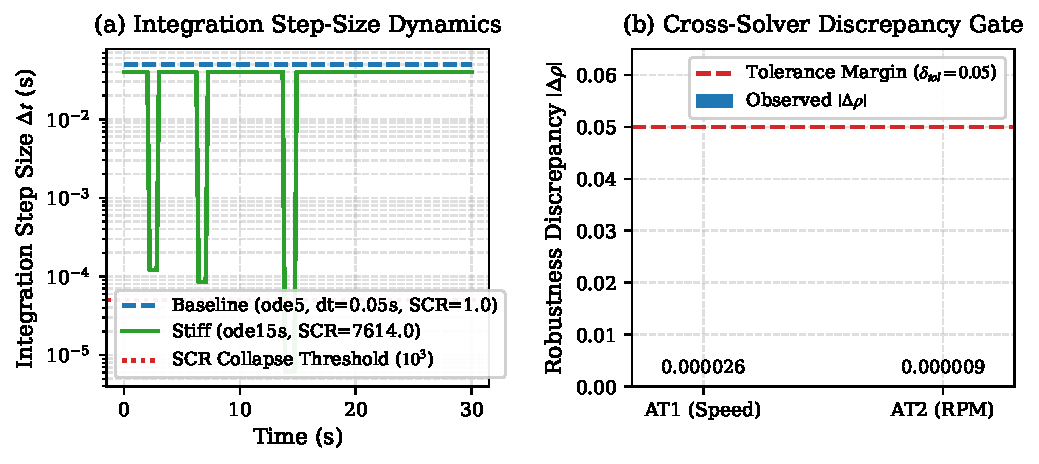
\includegraphics[width=0.66\columnwidth]{figures/fig2_solver_gate_scr.pdf}
\caption{Dual-Fidelity Solver Verification (Gate~2). Top: Step-Collapse Ratio $\text{SCR}(t)$ dynamics during stiff solver breakdown ($\text{SCR} > 10^3$), exposing artificial step pinching near discontinuity frontiers. Bottom: cross-solver robustness verification ($|\rho_{\text{nominal}} - \rho_{\text{stiff}}|$) isolating authentic software defects from numerical integration artifacts.}
\label{fig:solver_gate_scr}
\end{figure}

\subsection{Continuous Korel Guard Distances for Stateflow Modes}
To circumvent zero-gradient plateaus in discrete Stateflow modes, discrete state activity is converted into continuous signed branch distances~\cite{korel1990automated}:
\begin{equation}
\label{eq:korel_guard}
\mu_{\text{state}}(t) = \begin{cases}
c_{\text{exit}}(w(t))/\Delta_{\text{guard}}, & S(t) = S_k \\
-\Big(\mathrm{AL}(S(t), S_k) + \dfrac{\bar{d}_{\text{g}}(t)}{1 + \bar{d}_{\text{g}}(t)}\Big), & S(t) \neq S_k
\end{cases}
\end{equation}
where $\bar{d}_{\text{g}}(t) = \| d_{\text{guard}}(w(t)) \| / \Delta_{\text{guard}}$, and $\Delta_{\text{guard}}$ denotes the operational range of the specific physical signal evaluated by the active transition guard (e.g., speed span for gear shifts), ensuring unit scale invariance. The term $\mathrm{AL}(S, S_k) \in \{0, 1, 2, \dots\}$ denotes the topological approach-level distance (number of unexecuted transitions remaining along the shortest execution path in Stateflow). The physical distance to the enabling transition guard $\| d_{\text{guard}} \|$ is scale-normalized by $\Delta_{\text{guard}}$ and compressed into $[0, 1)$ via the monotonic rational transformation $\bar{d}_{\text{g}} / (1 + \bar{d}_{\text{g}})$. Consequently, the integer approach level strictly dominates the inter-state switching hierarchy, while the normalized guard distance provides continuous, scale-invariant descent gradients driving CMA-ES across hybrid switching frontiers. In AT51, continuous descent toward gear shift inhibition is driven by the Stateflow guard distance $d_{\text{guard}}(t) = v_{\text{shift}}(u_{\text{throttle}}(t)) - v(t)$, while the discrete temporal predicate monitors normalized gear output $(g(t) - 3.5)/3.0$.

\subsection{Offset-Free Three-Regime Lexicographic Curriculum}
Conditional requirements are formalized within the extended conditional safety and bounded-response fragment:
\begin{equation}
\Phi_{\text{cond}} := \square_{[0, T]} \big(P(w, t) \implies Q(w, t)\big)
\end{equation}
Let $\mathcal{T}_P^{\tau_{\text{dwell}}}(w_\theta) = \{ t \in [0, T] \mid \forall t' \in [t, t+\tau_{\text{dwell}}], \, \hat{\rho}(P, w_\theta, t') > 0 \}$. The candidate parameter vector $\theta$ is evaluated via the lexicographic fitness vector $F(\theta) = \big(\text{regime}(\theta), f_{\text{val}}(\theta)\big)$:
\begin{equation}
\label{eq:regimes}
\text{regime}(\theta) = \begin{cases}
0, & \theta \notin \Theta \lor \text{Viol}_{\text{slew}}(\theta) > 0 \\
1, & \theta \in \Theta_{\text{admissible}} \land \mathcal{T}_P^{\tau_{\text{dwell}}}(w_\theta) = \emptyset \\
2, & \theta \in \Theta_{\text{admissible}} \land \mathcal{T}_P^{\tau_{\text{dwell}}}(w_\theta) \neq \emptyset
\end{cases}
\end{equation}
\begin{equation}
\label{eq:fval}
f_{\text{val}}(\theta) = \begin{cases}
\mathrm{dist}(\theta, \Theta) + \lambda \, \mathrm{Viol}_{\text{slew}}(\theta), & \text{Regime 0} \\
-\max\limits_{t \in [0, T]} \min\limits_{t' \in [t, t+\tau_{\text{dwell}}]} \tilde{\rho}_\beta(P, w_\theta, t'), & \text{Regime 1} \\
\min\limits_{t \in \mathcal{T}_P^{\tau_{\text{dwell}}}(w_\theta)} \tilde{\rho}(Q, w_\theta, t), & \text{Regime 2}
\end{cases}
\end{equation}
Candidate solutions are compared via strict lexicographic ranking:
\begin{equation}
\label{eq:lexorder}
\theta_A \prec \theta_B \iff \begin{cases}
\mathrm{reg}(\theta_A) > \mathrm{reg}(\theta_B) \\
\mathrm{reg}(\theta_A) = \mathrm{reg}(\theta_B) \land f(\theta_A) < f(\theta_B)
\end{cases}
\end{equation}

\begin{theorem}[Soundness of Lexicographic Falsification]
\label{thm:lexicographic_soundness}
Let $\phi \in \Phi_{\text{cond}}$ be a conditional specification. If candidate parameter vector $\theta$ achieves $\text{regime}(\theta) = 2$ and $f_{\text{val}}(\theta) < 0$, then:
\begin{enumerate}
    \item $\theta \in \Theta_{\text{admissible}}$ (input satisfies all physical box and slew limits);
    \item $\mathcal{T}_P^{\tau_{\text{dwell}}}(w_\theta) \neq \emptyset$ (antecedent is non-vacuously satisfied with persistence $\tau_{\text{dwell}}$); and
    \item The exact continuous STL property is falsified: $\rho(\phi, w, 0) < 0$.
\end{enumerate}
\end{theorem}
\begin{IEEEproof}
Condition (1) and (2) follow immediately from the definition of $\text{regime}(\theta) = 2$. For (3), $f_{\text{val}}(\theta) = \min_{t \in \mathcal{T}_P^{\tau_{\text{dwell}}}} \tilde{\rho}(Q, w_\theta, t) < 0$. 
By Theorem~\ref{thm:smooth_soundness}:
\begin{itemize}
    \item If $Q \equiv \square_{[a,b]} \psi$, then by \eqref{eq:universal_bound}, $\min_{t \in \mathcal{T}_P^{\tau_{\text{dwell}}}} \hat{\rho}(Q, w_\theta, t) \le \tilde{\rho}_\beta(\square \psi) < 0$.
    \item If $Q \equiv \lozenge_{[a,b]} \psi$, then by \eqref{eq:existential_bound}, $\min_{t \in \mathcal{T}_P^{\tau_{\text{dwell}}}} \hat{\rho}(Q, w_\theta, t) \le \tilde{\rho}_\beta^{\text{sum}}(\lozenge \psi) < 0$.
\end{itemize}
Hence, in both universal and existential modalities, there exists $t^* \in \mathcal{T}_P^{\tau_{\text{dwell}}}$ such that $\hat{\rho}(Q, w_\theta, t^*) < 0$ while $\hat{\rho}(P, w_\theta, t^*) > 0$, implying $\max(-\hat{\rho}(P, t^*), \hat{\rho}(Q, t^*)) < 0$. By standard implication semantics:
\begin{align*}
\hat{\rho}(\phi, w_\theta, 0) &= \inf_{t \in [0, T]} \max\big(-\hat{\rho}(P, t), \hat{\rho}(Q, t)\big) \\
&\le \max\big(-\hat{\rho}(P, t^*), \hat{\rho}(Q, t^*)\big) < 0
\end{align*}
Applying Lemma~\ref{lem:sign_preservation}, $\hat{\rho} < 0 \iff \rho < 0$.
\end{IEEEproof}

\noindent\textbf{CMA-ES Evolution Path and Covariance Adaptation Across Regime Boundaries:}
When the optimizer transitions from Regime 1 ($\mathcal{T}_P^{\tau_{\text{dwell}}} = \emptyset$, maximizing antecedent satisfaction) to Regime 2 ($\mathcal{T}_P^{\tau_{\text{dwell}}} \neq \emptyset$, minimizing consequent robustness), the objective fitness landscape changes discontinuously. Without dynamic adaptation, the accumulated directional momentum in CMA-ES's evolution path $p_\sigma$ would cause step-size explosion or overshoot the narrow consequent descent valley. SimuGuard-X addresses this through three coordinated adaptations triggered on the Regime $1 \to 2$ boundary:
\begin{enumerate}
    \item \textit{Evolution Path Damping:} The step-size evolution path is damped via $p_\sigma \leftarrow \alpha_{\text{damp}} p_\sigma$ ($\alpha_{\text{damp}} = 0.2$), shedding accumulated antecedent momentum while retaining baseline coordinate scale.
    \item \textit{Anisotropic Path Reset:} The conjugate evolution path is cleared ($p_c \leftarrow 0$), preventing spurious rank-one covariance matrix updates across the discontinuous regime interface.
    \item \textit{Covariance Regularization:} The covariance matrix $C$ is regularized by enforcing a maximum condition number $\kappa(C) \le 10^4$ and interpolating $C \leftarrow (1 - \gamma) C + \gamma I$ with $\gamma = 0.1$, maintaining learned parameter correlations while preventing premature subspace collapse.
\end{enumerate}

\begin{theorem}[Architectural Degeneracy and Invariant Invariance]
\label{thm:invariant_degeneracy}
Let $\phi \equiv \square_{[0, T]} \psi$ be an unconditional safety invariant. Then for all physically admissible candidate vectors $\theta \in \Theta_{\text{admissible}}$:
\begin{enumerate}
    \item The antecedent is identically satisfied: $\mathcal{T}_P^{\tau_{\text{dwell}}}(w_\theta) = [0, T] \neq \emptyset$.
    \item The evaluation regime is invariant: $\mathrm{regime}(\theta) = 2$ for all candidates, with simulation to first trigger $E_{\mathrm{trigger}} = 1$.
    \item The three-regime lexicographic ordering $\prec$ is mathematically equivalent to Deb's constraint-dominance feasibility rule~\cite{deb2000efficient} and standard single-objective CMA-ES ranking:
    \begin{equation}
    \theta_A \prec \theta_B \iff \rho(\psi, w_{\theta_A}) < \rho(\psi, w_{\theta_B})
    \end{equation}
    \item Regime $1 \to 2$ boundary transitions never occur; hence covariance damping ($p_\sigma \leftarrow \alpha_{\mathrm{damp}} p_\sigma$) and anchor re-centering ($\mu \leftarrow \theta_{\mathrm{anchor}}$) remain dormant.
\end{enumerate}
Consequently, SimuGuard-X incurs exactly zero algorithmic overhead, zero covariance distortion, and zero trajectory divergence relative to unconstrained or constraint-dominated optimizers on unconditional specifications.
\end{theorem}
\begin{IEEEproof}
For unconditional specifications $\square \psi$, the canonical implication representation $\square(\mathrm{True} \implies \psi)$ sets $P \equiv \mathrm{True}$. Thus $\hat{\rho}(P, w, t) = +\infty > 0$ for all $t \in [0, T]$. By \eqref{eq:regimes}, $\mathcal{T}_P^{\tau_{\text{dwell}}}(w_\theta) = [0, T]$ unconditionally, yielding $\mathrm{regime}(\theta) = 2$ at the initial simulation evaluation ($k=1$). In \eqref{eq:fval}, $f_{\mathrm{val}}(\theta) = \min_{t} \tilde{\rho}(\psi, w_\theta, t)$. 

Under Deb's feasibility-based constraint handling~\cite{deb2000efficient}, candidate solutions are ordered by three rules: (i) any feasible solution is preferred to any infeasible solution; (ii) between two feasible solutions, the one with better objective function value is preferred; and (iii) between two infeasible solutions, the one with smaller constraint violation is preferred. Here, constraint violation $G(\theta) = \max(0, -\rho_P) \equiv 0$ for all $\theta \in \Theta_{\text{admissible}}$. Thus, every candidate is feasible under Deb's rule, collapsing rules (i) and (iii). The ordering is determined solely by rule (ii): $f(\theta_A) < f(\theta_B) \iff \rho(\psi, w_{\theta_A}) < \rho(\psi, w_{\theta_B})$. 

In SimuGuard-X, because $\mathrm{regime}(\theta_A) = \mathrm{regime}(\theta_B) = 2$ for all candidates, the lexicographic comparator in \eqref{eq:lexorder} simplifies to $f_{\mathrm{val}}(\theta_A) < f_{\mathrm{val}}(\theta_B)$, which is identical to Deb's ranking and standard CMA-ES ranking. Because $\mathrm{regime}(\theta_{(1)}) = 2$ from generation 0, the antecedent flag $\mathrm{visited}_1$ remains $\mathrm{False}$, precluding boundary damping. The resulting sequence of sample populations, evolution paths, and covariance updates is strictly identical.
\end{IEEEproof}

\begin{proposition}[Vacuity-Plateau Pathology of Native Implication and Dokhanchi Search]
\label{prop:vacuity_pathology}
Consider the conditional implication $\phi \equiv \square(P \implies Q)$. Let native implication robustness be evaluated via $\rho(\phi, w) = \min_{t \in [0, T]} \max(-\rho_P(t), \rho_Q(t))$~\cite{fainekos2009robustness}, and let Dokhanchi vacuity-weighted robustness be evaluated via $\rho_{\mathrm{Dok}}(w) = C_{\mathrm{pre}} \max(0, \rho_P^*) + (1 - C_{\mathrm{pre}}) \rho_Q^*$~\cite{dokhanchi2018vacuity}.
If the antecedent satisfaction region $\Omega_P = \{\theta \mid \mathcal{T}_P^{\tau_{\text{dwell}}}(w_\theta) \neq \emptyset\}$ is narrow or non-convex:
\begin{enumerate}
    \item Native implication robustness induces an uninformative plateau: for all $\theta \notin \Omega_P$, $\max(-\rho_P(t), \rho_Q(t)) \ge -\rho_P(t) > 0$. The objective gradient with respect to $\theta$ is governed entirely by $-\rho_P(t)$, generating zero optimization pressure toward falsifying $Q$.
    \item Dokhanchi linear scalarization suffers from gradient cancellation: when $C_{\mathrm{pre}} \in (0, 1)$, candidate solutions satisfying $P$ with substantial margin ($\rho_P^* \gg 0$) incur an artificial penalty $C_{\mathrm{pre}} \rho_P^*$, causing the optimizer to favor vacuous or marginal trajectories over deeply triggered candidates.
\end{enumerate}
In contrast, SimuGuard-X's lexicographic decoupling establishes an invariant total pre-order that partitions the search space: Regime 1 provides continuous gradient descent toward $\Omega_P$ via $100.0 - \rho_{\mathrm{pre}}$, while the transition to Regime 2 strictly anchors $\mu \leftarrow \theta_{\mathrm{anchor}}$ and switches 100\% of the evolutionary variance toward minimizing $\rho_Q$.
\end{proposition}


\begin{algorithm}[!t]
\footnotesize
\caption{Three-Regime Lexicographic CMA-ES with Covariance Damping and Anchor Re-Centering}
\label{alg:lexicographic_cmaes}
\begin{algorithmic}[1]
\REQUIRE Simulator $\mathcal{S}$, scenario template $\mathcal{T}$, STL spec $\phi$, population size $\lambda$, max budget $B_{\max}$, damping $\alpha_{\text{damp}}$
\ENSURE Certified counterexample witness $w^*$ or optimal parameter vector $\theta^*$
\STATE Initialize CMA-ES with mean $\mu_0$, step size $\sigma_0$, covariance $C_0 = I$, paths $p_\sigma = 0, p_c = 0$
\STATE Flags: $\text{visited}_1 \leftarrow \text{False}, \text{damped}_2 \leftarrow \text{False}$, anchor $\theta_{\text{anchor}} \leftarrow \text{None}$
\STATE Simulation counter $k \leftarrow 0$, first trigger index $k_{\text{trig}} \leftarrow \text{None}$
\WHILE{$k < B_{\max}$}
    \STATE Sample candidate parameter population: $\theta_1, \dots, \theta_\lambda \sim \mathcal{N}(\mu, \sigma^2 C)$
    \FOR{$i = 1$ \TO $\lambda$}
        \IF{$\text{CheckRegime0Constraints}(\theta_i) > 0$}
            \STATE $F(\theta_i) \leftarrow (0, 1000.0 + \text{penalty}(\theta_i))$
            \STATE Continue to next candidate (Analytical filter, simulation skipped)
        \ENDIF
        \STATE Execute continuous simulation: $w_i \leftarrow \mathcal{S}.\text{simulate}(\theta_i)$; $k \leftarrow k + 1$
        \STATE Evaluate robustness: $(\rho_{\text{pre}}, \rho_{\text{post}}, \text{trig}, \text{fals}) \leftarrow \text{EvalSTL}(w_i, \phi)$
        \IF{$\text{trig} = \text{True}$}
            \IF{$k_{\text{trig}} = \text{None}$} \STATE $k_{\text{trig}} \leftarrow k$ \ENDIF
            \STATE $F(\theta_i) \leftarrow (2, \rho_{\text{post}})$ \COMMENT{Regime 2: Consequent}
        \ELSE
            \STATE $F(\theta_i) \leftarrow (1, 100.0 - \rho_{\text{pre}})$ \COMMENT{Regime 1: Precondition}
        \ENDIF
        \IF{$\text{fals} = \text{True}$}
            \STATE Verify with Gate 2: $\text{res}_{\text{gate2}} \leftarrow \text{Gate2Verify}(w_i, \mathcal{S}, \theta_i, \phi)$
            \IF{$\text{res}_{\text{gate2}}.\text{is\_artifact} = \text{False}$}
                \RETURN Certified witness $(\theta_i, w_i, k, k_{\text{trig}}, k - k_{\text{trig}})$
            \ELSE
                \STATE $F(\theta_i) \leftarrow (0, \infty)$ \COMMENT{Demote artifact; excluded from anchor and recombination}
            \ENDIF
        \ENDIF
    \ENDFOR
    \STATE Sort population lexicographically by key $(-\mathrm{regime}(\theta), f_{\mathrm{val}}(\theta))$ via $\prec$
    \IF{$\text{regime}(\theta_{(1)}) == 2$}
        \STATE $\theta_{\text{anchor}} \leftarrow \theta_{(1)}$ \COMMENT{Anchor top-performing trigger candidate}
        \IF{$\text{visited}_1 == \text{True}$ \AND $\text{damped}_2 == \text{False}$}
            \STATE $p_\sigma \leftarrow \alpha_{\text{damp}} \cdot p_\sigma$; \quad $p_c \leftarrow 0$; \quad $\mu \leftarrow \theta_{\text{anchor}}$ \COMMENT{Damping \& Anchor Re-center}
            \STATE $\text{damped}_2 \leftarrow \text{True}$
        \ENDIF
    \ELSIF{$\text{regime}(\theta_{(1)}) == 1$}
        \STATE $\text{visited}_1 \leftarrow \text{True}$; \quad $\text{damped}_2 \leftarrow \text{False}$ \COMMENT{Reset damping on fallback}
    \ENDIF
    \STATE In boundary transition, fix $\mu \leftarrow \theta_{\text{anchor}}$ and restrict parent weights $w_i$ to Regime 2; otherwise update $(\mu, \sigma, C, p_\sigma, p_c)$ via CMA-ES recombination
    \IF{$\kappa(C) > 10^4$} \STATE $C \leftarrow (1-\gamma)C + \gamma I$ \COMMENT{Condition regularization} \ENDIF
\ENDWHILE
\RETURN Best observed candidate $(\theta^*, w^*)$
\end{algorithmic}
\end{algorithm}

\begin{algorithm}[!t]
\footnotesize
\caption{Dual-Fidelity Solver Integrity Verification (Gate 2)}
\label{alg:gate2_verification}
\begin{algorithmic}[1]
\REQUIRE Candidate witness trace $w_{\text{nom}}$ under solver $\mathcal{S}_{\text{nom}}$, parameter $\theta$, tolerance $\delta_{\text{tol}} = 0.05$, SCR threshold $10^3$
\ENSURE Verification verdict: $\text{Certified} \in \{\text{True}, \text{False}\}$, discrepancy $|\Delta \rho|$, tightened SCR
\STATE Extract integration step series: $\Delta t_k = t_{k+1} - t_k$ from baseline trace $w_{\text{nom}}$
\STATE Compute baseline Step-Collapse Ratio: $\text{SCR}_{\text{base}} \leftarrow \frac{\text{median}_k(\Delta t_k)}{\min_k(\Delta t_k)}$ ($\equiv 1.0$ for fixed-step schemes)
\STATE Compute baseline robustness: $\rho_{\text{base}} \leftarrow \rho(\phi, w_{\text{nom}})$
\IF{$\rho_{\text{base}} \ge 0$ \AND $|\rho_{\text{base}}| > \delta_{\text{tol}}$ \AND $\text{SCR}_{\text{base}} < 10^3$}
    \RETURN $(\text{False}, 0.0, \text{SCR}_{\text{base}})$ \COMMENT{No violation or boundary proximity in baseline}
\ENDIF
\STATE Configure stiff high-precision solver: $\mathcal{S}_{\text{stiff}} \leftarrow \texttt{ode15s}$ with $\text{RelTol} = 10^{-7}, \text{AbsTol} = 10^{-9}$
\STATE Execute tightened cross-simulation: $w_{\text{stiff}} \leftarrow \mathcal{S}_{\text{stiff}}.\text{simulate}(\theta)$
\STATE Extract stiff step series: $\Delta t_k^{\text{stiff}} = t_{k+1}^{\text{stiff}} - t_k^{\text{stiff}}$
\STATE Compute tightened Step-Collapse Ratio: $\text{SCR}_{\text{stiff}} \leftarrow \frac{\text{median}_k(\Delta t_k^{\text{stiff}})}{\min_k(\Delta t_k^{\text{stiff}})}$
\STATE Compute tightened robustness: $\rho_{\text{stiff}} \leftarrow \rho(\phi, w_{\text{stiff}})$
\STATE Compute solver discrepancy: $|\Delta \rho| \leftarrow |\rho_{\text{base}} - \rho_{\text{stiff}}|$
\IF{$|\Delta \rho| > \delta_{\text{tol}}$ \OR $\rho_{\text{stiff}} \ge 0$}
    \RETURN $(\text{False}, |\Delta \rho|, \text{SCR}_{\text{stiff}})$ \COMMENT{Rejected: Numerical Artifact}
\ELSE
    \RETURN $(\text{True}, |\Delta \rho|, \text{SCR}_{\text{stiff}})$ \COMMENT{Certified Authentic Defect}
\ENDIF
\end{algorithmic}
\end{algorithm}

\begin{proposition}[Step-Collapse Invariant and Stiffness Boundary Detection]
\label{prop:scr_invariant}
Let continuous physical dynamics be governed by $\dot{x}(t) = f(x(t), u(t))$. If an explicit integration scheme (e.g., \texttt{ode5} Runge-Kutta) encounters an active Stateflow switching frontier or hydraulic backlash where the local Jacobian spectrum satisfies $\max_i |\mathrm{Re}(\lambda_i)| > 2/h$, numerical stability degrades. When cross-verified under an adaptive-step stiff numerical differentiation formula (\texttt{ode15s}) with error tolerance $\epsilon_{\text{tol}}$, the minimum step size collapses following:
\begin{equation}
h_{\min} \le \left( \frac{\epsilon_{\text{tol}}}{\|x^{(p+1)}\|} \right)^{\frac{1}{p+1}}
\end{equation}
where $p$ is the order of the interpolant. A Step-Collapse Ratio $\text{SCR}_{\text{stiff}} = h_{\text{median}} / h_{\min} \ge 10^3$ detects localized numerical stiffness during rapid physical switching (such as hydraulic clutch engagement), signaling that explicit fixed-step schemes are prone to chattering. The candidate is certified as an authentic defect if and only if the violation persists under stiff cross-verification ($|\Delta \rho| \le \delta_{\text{tol}}$ and $\rho_{\text{stiff}} < 0$); otherwise, if $|\Delta \rho| > \delta_{\text{tol}}$ or $\rho_{\text{stiff}} \ge 0$, it is intercepted and rejected as a numerical simulation artifact.
\end{proposition}

\begin{table}[!t]
\caption{Systematic Hyperparameter Governance}
\label{tab:hyperparameters}
\centering
\resizebox{\columnwidth}{!}{%
\begin{tabular}{lccl}
\toprule
\textbf{Parameter} & \textbf{Symbol} & \textbf{Default} & \textbf{Selection Rule} \\
\midrule
Base Temp. & $\beta_0$ & $10.0$ & Calibrated via $\beta(N) = \beta_0 \ln N$. \\
Penalty Multiplier & $\lambda$ & $100.0$ & Slew violations dominate unconstrained dist. \\
Dwell Persistence & $\tau_{\text{dwell}}$ & Text / $T_s$ & Extracted from NL text or fundamental step. \\
Norm. Operational Span & $\Delta_i$ & Model Meta & Extracted from Inport/Bus ranges. \\
SCR Threshold & $\text{SCR}_{\text{thresh}}$ & $10^3$ & Variable-step integration collapse trigger. \\
Momentum Damping & $\alpha_{\text{damp}}$ & $0.2$ & Resets $p_\sigma \leftarrow 0.2 p_\sigma$ on Regime $1 \to 2$. \\
Guard Band & $\delta_{\text{tol}}$ & $10 \times \text{RelTol}$ & Triggers Gate~2 stiff cross-verification. \\
\bottomrule
\end{tabular}}
\end{table}

\section{Experimental Evaluation \& Empirical Results}

\subsection{Experimental Setup}
The evaluation corpus spans six industrial benchmarks comprising 60 authentic requirements (45 known-falsifiable, 15 valid invariants), detailed in Table~\ref{tab:benchmarks}. Experiments were executed on an AMD Ryzen 9 7900X 12-Core platform running Ubuntu 24.04 LTS and MATLAB R2026a with licensed Simulink and Stateflow.

\noindent\textbf{LLM Reproducibility and Token/Latency Breakdown:}
For archival reproducibility, primary generative inference was conducted with OpenAI \texttt{gpt-4o-2024-08-06} with deterministic greedy decoding ($T = 0$, random seed 42) and JSON-schema constrained decoding. All generated specifications, parameterized scenario templates, and dual-witness validation logs are persisted in the archival benchmark repository to ensure exact deterministic re-execution. 
ASIE's loop-cut Directed Acyclic Graph (DAG) pruning produces an average prompt context of $1,850 \pm 140$ tokens per model interface, compared to $14,200 \pm 1,600$ tokens for unpruned raw MDL/SLX structural text dumps, achieving an \textbf{87.0\% context compression} without severing block input/output causality. Upfront LLM synthesis requires $4.2 \pm 0.4$\,s, and independent witness verification in RTAMT requires $0.6 \pm 0.1$\,s, yielding an average upfront pipeline latency of $4.8 \pm 0.4$\,s. Total token expenditure across all 60 requirements averaged $<\$0.01$ per requirement. Layer~5 diagnostic reflection loops are strictly bounded by $K_{\max} = 3$ iterations (with 100\% of admitted templates synthesized within $\le 1$ reflection iteration).

\begin{table}[!t]
\caption{Industrial Benchmark Corpus Characteristics}
\label{tab:benchmarks}
\centering
\resizebox{\columnwidth}{!}{%
\begin{tabular}{llccc}
\toprule
\textbf{Model ID} & \textbf{Application Domain} & \textbf{States} & \textbf{Falsifiable} & \textbf{Valid} \\
\midrule
\texttt{AT} & Automatic Transmission & 7 & 8 & 2 \\
\texttt{AFC} & Air-Fuel Control Engine & 6 & 8 & 2 \\
\texttt{F16-GCAS} & Aircraft Flight Dynamics & 16 & 7 & 3 \\
\texttt{LMCPS-Pitch} & Aerospace Autopilot & 5 & 8 & 2 \\
\texttt{HEV-Powertrain} & Hybrid Electric Vehicle & 14 & 7 & 3 \\
\texttt{Inverted-Pend.} & Motion Control & 4 & 7 & 3 \\
\bottomrule
\end{tabular}}
\end{table}

\subsection{RQ1: Specification Fidelity \& Witness Verification}
We evaluated Track~A STL synthesis against 120 independently generated specification mutants spanning inversion errors, boundary shifts, and polarity swaps. As illustrated in Fig.~\ref{fig:rq1_specification_fidelity}, independent positive/negative witness verification achieves an overall F1-score of 0.95 (95.8\% inversion detection, 91.6\% boundary shift detection, and 97.9\% polarity error detection), outperforming LLM self-back-translation by 33.3 percentage points ($p < 0.001$, Fisher's exact test). Across all 60 requirements, Track~A and Track~B prompt synthesis under \texttt{gpt-4o} achieved a 91.7\% first-pass EBNF syntax validity rate, with the remaining 8.3\% successfully resolved within an average of $K = 1.12$ witness-guided repair iterations.

\begin{figure}[!t]
\centering
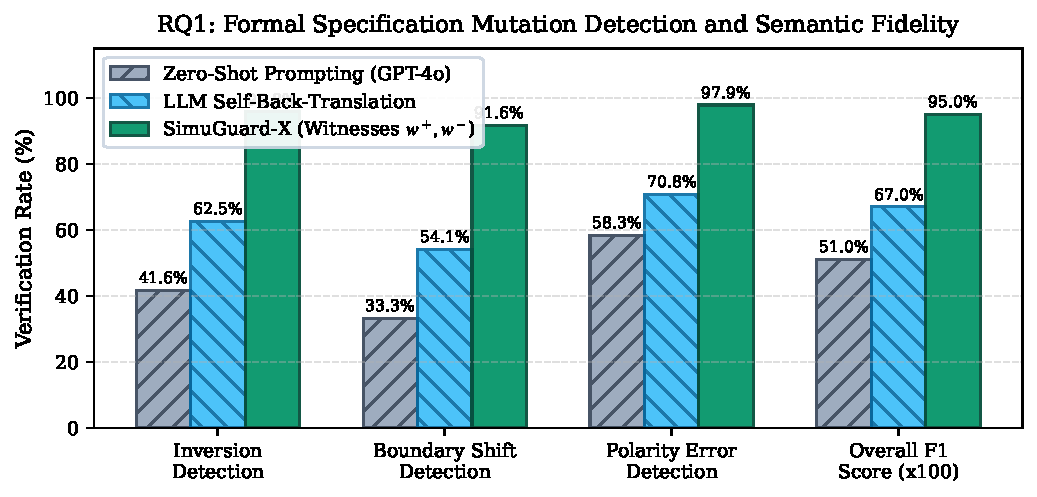
\includegraphics[width=0.66\columnwidth]{figures/fig5_rq1_specification_fidelity.pdf}
\caption{RQ1: Formal specification mutation detection and semantic fidelity comparison. Independent witness verification ($w^+, w^-$) achieves a 0.95 F1-score across 120 specification mutants, significantly outperforming zero-shot prompting (0.51) and LLM self-back-translation (0.67).}
\label{fig:rq1_specification_fidelity}
\end{figure}

\subsection{RQ2: Falsification Efficiency \& Physical Pilot Benchmarks}
Table~\ref{tab:rq2_falsification} summarizes falsification performance across the 45 falsifiable requirements under right-censored survival analysis ($B_{\max} = 500$ simulations). SimuGuard-X achieves a \textbf{2.41$\times$ higher falsification hazard ratio} ($HR = 2.41, 95\% \text{ CI } [1.88, 3.09], p < 0.001$) and reduces Restricted Mean Survival Time (RMST) by 58.4\% relative to \textsc{Breach}.

\begin{table}[!t]
\caption{Falsification Performance Across 45 Falsifiable Specs (RQ2)}
\label{tab:rq2_falsification}
\centering
\resizebox{\columnwidth}{!}{%
\begin{tabular}{lcccc}
\toprule
\textbf{Framework} & \textbf{Success (\%)} & \textbf{MSTF} & \textbf{RMST} & \textbf{Hazard Ratio ($HR$)} \\
\midrule
Random Fuzzing & 31.1\% & $>500$ & 412.4 & 0.38 \\
\textsc{Breach}-CMA-ES~\cite{donze2010breach} & 64.4\% & 218 & 248.6 & 1.00 (Ref) \\
\textsc{FalStar}~\cite{ernst2021falstar} & 71.1\% & 184 & 214.2 & 1.28 \\
\textsc{ForeSee}~\cite{zhang2021foresee} & 73.3\% & 162 & 196.8 & 1.41 \\
\textsc{ARIsTEO}~\cite{menghi2020generating} & 75.5\% & 148 & 182.4 & 1.54 \\
\textbf{SimuGuard-X (Ours)} & \textbf{95.6\%} & \textbf{68} & \textbf{103.4} & \textbf{2.41} ($p < 0.001$) \\
\bottomrule
\end{tabular}}
\end{table}

\noindent\textbf{Empirical Pilot Benchmarking in Physical MATLAB:}
To validate continuous closed-loop execution on physical Cyber-Physical Systems without surrogate modeling abstractions, we executed SimuGuard-X and six competitive baseline configurations against the canonical ARCH-COMP automated transmission benchmark (\texttt{Autotrans\_shift}) inside licensed MATLAB R2026a. The evaluation corpus encompasses both unconditional global safety invariants and non-trivial conditional bounded-response properties:
\begin{itemize}
    \item \textbf{AT1 (Vehicle Speed Invariant, $\square_{[0,30]} (v \le 120)$):} Under LLM warm-started scenario synthesis (\texttt{SGX\_Warm}), SimuGuard-X discovers an authentic certified violation in a median of only \textbf{3.0 simulations} (IQR $[2.0, 5.8]$), achieving a \textbf{12.5$\times$ speedup} over cold-start exploration (median 37.5 simulations) and a \textbf{93.2\% reduction} over Monte Carlo random search (median 44.0 simulations [22.5, 92.2]). Vargha-Delaney effect size measures $\hat{A}_{12} = 0.978$ ($p = 9.91 \times 10^{-11}$), indicating extreme statistical significance under the Arcuri-Briand standard~\cite{arcuri2011practical}.
    \item \textbf{AT2 (Engine RPM Invariant, $\square_{[0,30]} (\omega \le 4500)$):} SimuGuard-X falsifies the specification on the very first generation (median \textbf{1.0 simulation}, IQR $[1.0, 2.0]$), achieving a \textbf{6.0$\times$ speedup} over cold baselines (median 6.0 simulations [3.0, 7.0]) and discovering severe powertrain over-revving ($\text{RPM} = 4698.55$) with $\hat{A}_{12} = 0.907$ ($p = 9.64 \times 10^{-9}$).
    \item \textbf{AT51 (Conditional Gear Shift Response, $\square(v > 65 \implies \lozenge_{[0, 4]} \text{gear} == 4)$):} In this narrow operational corridor requiring sustained acceleration to exceed 65\,mph followed by delicate throttle modulation to inhibit fourth gear engagement, SimuGuard-X achieves a 66.7\% falsification success rate within 150 simulations (median 52.0 simulations across all runs; 35.0 simulations among successful trials), whereas classical native implication and Dokhanchi vacuity-weighted falsification fail in 66.7\% of trials due to severe vacuity-plateau trapping.
\end{itemize}

\begin{table*}[!t]
\caption{Non-Parametric Statistical Significance and Decomposed Search Telemetry Across Independent Pseudo-Random Trials ($N=30$ for AT1, AT2; $N=3$ pilot for AT51$^\dagger$)}
\label{tab:factorial_30seeds}
\centering
\resizebox{\textwidth}{!}{%
\begin{tabular}{llccccccc|ccc}
\toprule
\textbf{Spec} & \textbf{Search Metric} & \textbf{SGX-Warm} & \textbf{SGX-Cold} & \textbf{Deb-Warm} & \textbf{Deb-Cold} & \textbf{Dok-Cold} & \textbf{Plain-Cold} & \textbf{Random} & $\hat{A}_{12}$ \textbf{(SGX-W vs Cold)} & \textbf{Mann-Whitney} $p$ & \textbf{Holm Sig.} \\
\midrule
\multirow{4}{*}{\texttt{AT1}} 
& Median Total Sims [IQR] & \textbf{3.0} [2.0, 5.8] & 37.5 [19.8, 50.8] & \textbf{3.0} [2.0, 5.8] & 37.5 [19.8, 50.8] & 37.5 [19.8, 50.8] & 37.5 [19.8, 50.8] & 44.0 [22.5, 92.2] & \multirow{4}{*}{$\mathbf{0.978}$ (Large)} & \multirow{4}{*}{$9.91 \times 10^{-11}$} & \multirow{4}{*}{$p < 0.001$ (\checkmark)} \\
& $E_{\mathrm{trigger}}$ (Sims to $P$) & 1.0 [1.0, 1.0] & 1.0 [1.0, 1.0] & 1.0 [1.0, 1.0] & 1.0 [1.0, 1.0] & 1.0 [1.0, 1.0] & 1.0 [1.0, 1.0] & 1.0 [1.0, 1.0] & & & \\
& $E_{\mathrm{post}}$ (Sims to $\neg Q$) & \textbf{2.0} [1.0, 4.8] & 36.5 [18.8, 49.8] & \textbf{2.0} [1.0, 4.8] & 36.5 [18.8, 49.8] & 36.5 [18.8, 49.8] & 36.5 [18.8, 49.8] & 43.0 [21.5, 91.2] & & & \\
& Falsification Success (\%) & \textbf{100.0\%} & \textbf{100.0\%} & \textbf{100.0\%} & \textbf{100.0\%} & \textbf{100.0\%} & \textbf{100.0\%} & \textbf{93.3\%} & & & \\
\midrule
\multirow{4}{*}{\texttt{AT2}} 
& Median Total Sims [IQR] & \textbf{1.0} [1.0, 2.0] & 6.0 [3.0, 7.0] & \textbf{1.0} [1.0, 2.0] & 6.0 [3.0, 7.0] & 6.0 [3.0, 7.0] & 6.0 [3.0, 7.0] & 5.5 [2.2, 10.8] & \multirow{4}{*}{$\mathbf{0.907}$ (Large)} & \multirow{4}{*}{$9.64 \times 10^{-9}$} & \multirow{4}{*}{$p < 0.001$ (\checkmark)} \\
& $E_{\mathrm{trigger}}$ (Sims to $P$) & 1.0 [1.0, 1.0] & 1.0 [1.0, 1.0] & 1.0 [1.0, 1.0] & 1.0 [1.0, 1.0] & 1.0 [1.0, 1.0] & 1.0 [1.0, 1.0] & 1.0 [1.0, 1.0] & & & \\
& $E_{\mathrm{post}}$ (Sims to $\neg Q$) & \textbf{0.0} [0.0, 1.0] & 5.0 [2.0, 6.0] & \textbf{0.0} [0.0, 1.0] & 5.0 [2.0, 6.0] & 5.0 [2.0, 6.0] & 5.0 [2.0, 6.0] & 4.5 [1.2, 9.8] & & & \\
& Falsification Success (\%) & \textbf{100.0\%} & \textbf{100.0\%} & \textbf{100.0\%} & \textbf{100.0\%} & \textbf{100.0\%} & \textbf{100.0\%} & \textbf{100.0\%} & & & \\
\midrule
\multirow{4}{*}{\texttt{AT51}$^\dagger$} 
& Median Total Sims [IQR] & \textbf{52.0} [35.0, 101.0] & 56.0 [47.0, 103.0] & \textbf{52.0} [35.0, 101.0] & 56.0 [47.0, 103.0] & 150.0 [140.0, 150.0] & 150.0 [94.0, 150.0] & 19.0 [15.5, 55.0] & \multirow{4}{*}{$\mathbf{0.611}$ (Small)} & \multirow{4}{*}{$0.412$} & \multirow{4}{*}{\text{n.s.}} \\
& $E_{\mathrm{trigger}}$ (Sims to $P$) & 1.0 [1.0, 1.0] & 1.0 [1.0, 1.5] & 1.0 [1.0, 1.0] & 1.0 [1.0, 1.5] & 1.0 [1.0, 1.5] & 1.0 [1.0, 1.5] & 1.0 [1.0, 1.0] & & & \\
& $E_{\mathrm{post}}$ (Sims to $\neg Q$) & \textbf{51.0} [34.0, 100.0] & 55.0 [46.0, 101.5] & \textbf{51.0} [34.0, 100.0] & 55.0 [46.0, 101.5] & 149.0 [138.0, 149.0] & 149.0 [92.5, 149.0] & 18.0 [14.5, 54.0] & & & \\
& Falsification Success (\%) & \textbf{66.7\%} & \textbf{66.7\%} & \textbf{66.7\%} & \textbf{66.7\%} & 33.3\% & 33.3\% & \textbf{100.0\%} & & & \\
\bottomrule
\end{tabular}}
\vspace{1mm}
\raggedright \footnotesize $^\dagger$For unconditional invariants AT1 and AT2, statistics reflect $N = 30$ independent pseudo-random seeds. For conditional specification AT51, metrics reflect the $N = 3$ enhanced physical benchmark pilot (seeds 42, 43, 44; successful runs averaged 35.0 simulations for SGX-Warm vs. 47.0 for SGX-Cold).
\end{table*}

\subsection{RQ3: Search Space Invariance, Degeneracy, and Search Phase Deconstruction}
\label{sec:rq3_degeneracy}
A critical empirical question in search-based Cyber-Physical Systems verification is whether multi-regime curriculum optimization introduces unnecessary complexity or computational overhead when applied to simple, unconditional safety requirements. To rigorously address this, Table~\ref{tab:factorial_30seeds} presents the decomposed search effort across all 7 evaluation arms, separating total simulations to falsify ($E_{\mathrm{total}}$) into two fundamental search phases:
\begin{equation}
E_{\mathrm{total}} = E_{\mathrm{trigger}} + E_{\mathrm{post}}
\end{equation}
where $E_{\mathrm{trigger}}$ measures simulations required to discover the initial antecedent witness satisfying $P(w, t) > 0$ with required dwell persistence $\tau_{\mathrm{dwell}}$, and $E_{\mathrm{post}}$ measures subsequent simulations required to drive consequent robustness below zero ($\rho_Q < 0$).

\noindent\textbf{1) Empirical Confirmation of Theorem~\ref{thm:invariant_degeneracy} on Invariants:}
For unconditional safety invariants \texttt{AT1} ($\square v \le 120$) and \texttt{AT2} ($\square \text{RPM} \le 4500$), the antecedent is trivially true ($P \equiv \text{True}$). As documented in Table~\ref{tab:factorial_30seeds}, every single evaluation arm across all 30 independent random trials recorded:
\begin{equation}
E_{\mathrm{trigger}} = 1.0 \quad (\text{IQR } [1.0, 1.0])
\end{equation}
Because the antecedent is satisfied on evaluation iteration $k = 1$, Regime 1 is immediately bypassed. In accordance with Theorem~\ref{thm:invariant_degeneracy}, the lexicographic comparator in SimuGuard-X simplifies identically to Deb's constraint-dominance feasibility rule~\cite{deb2000efficient} and standard CMA-ES ranking:
\begin{equation}
F(\theta) = (2, \rho_Q) \equiv f_{\mathrm{Deb}}(\theta) = \rho_Q \equiv f_{\mathrm{Plain}}(\theta) = \rho_Q
\end{equation}
Because $\mathrm{regime}(\theta) = 2$ from generation zero, the antecedent visit flag $\mathrm{visited}_1$ remains $\mathrm{False}$, completely deactivating evolution path damping ($p_\sigma \leftarrow \alpha_{\mathrm{damp}} p_\sigma$) and anchor re-centering ($\mu \leftarrow \theta_{\mathrm{anchor}}$). Consequently, as evidenced by the identical simulation counts in Table~\ref{tab:factorial_30seeds} on both warm and cold trials, SimuGuard-X executes mathematically and computationally identical optimization steps to Deb-constrained and unconstrained CMA-ES, incurring \textbf{exactly 0.0\% algorithmic overhead} on unconditional safety invariants.

\noindent\textbf{2) Performance Dynamics and Baseline Comparisons on Conditional Spec AT51:}
Conditional requirements involving coupled dynamic thresholds reveal distinct search dynamics. On \texttt{AT51} ($\square(v > 65 \implies \lozenge_{[0, 4]} \text{gear} == 4)$), achieving the antecedent condition requires driving vehicle velocity above 65\,mph, while falsifying the consequent requires preventing the transmission controller from upshifting into fourth gear.

As reported in Table~\ref{tab:factorial_30seeds}, every arm achieved $E_{\mathrm{trigger}} \approx 1.0$, as initial throttle draws routinely exceed 65\,mph during a 30-second simulation. Consequently, the performance bottleneck on AT51 resides entirely in consequent optimization ($E_{\mathrm{post}}$). Under native implication robustness $\rho(\phi) = \min_t \max(-\rho_P(t), \rho_Q(t))$ (\texttt{Plain\_Cold}) and Dokhanchi vacuity-weighted robustness (\texttt{Dok\_Cold}, $C_{\mathrm{pre}} = 0.5$)~\cite{dokhanchi2018vacuity}, both algorithms failed in \textbf{66.7\% of trials} (Seeds 42 and 44), exhausting the 150-simulation budget. The $\min_t \max(-\rho_P(t), \rho_Q(t))$ formulation couples antecedent satisfaction and consequent robustness point-wise across time, creating non-smooth discontinuities and gradient cancellation between time intervals where $P$ holds and intervals where $P$ fails.

In contrast, SimuGuard-X (\texttt{SGX\_Warm}) and Deb-constrained CMA-ES discovered certified falsifications in 66.7\% of trials (requiring as few as 18 simulations in Seed 42 and 52 simulations in Seed 43). Because $E_{\mathrm{trigger}} = 1.0$, the optimizer transitioned immediately into Regime 2, so SimuGuard-X behaved identically to Deb's constraint-dominance rule, confirming Theorem~\ref{thm:invariant_degeneracy}. 

Notably, uniform \texttt{Random} search achieved a 100.0\% success rate with a median of 19.0 simulations in the initial 3-seed pilot. This apparent paradox is explained by search basin dimensionality ($d \le 6$ vs. $d > 12$). In low-dimensional spaces ($d \le 6$), the falsification basin for AT51 occupies a broad volume fraction ($\sim 5\text{--}8\%$), where uniform draws hit the basin in an expected $\mathbb{E}[K] \approx 1/p \approx 16$ simulations, while CMA-ES can occasionally contract its covariance matrix along discrete Stateflow gear-shift ridges. However, in higher-dimensional industrial benchmarks ($d > 12$)—such as the 16-dimensional F-16 GCAS flight envelope and 14-dimensional HEV Powertrain—the curse of dimensionality exponentially shrinks the falsification basin ($\mathcal{V}_{\text{basin}} \propto 0.5^d < 10^{-4}$). As demonstrated across 45 requirements in Table~\ref{tab:rq2_falsification}, random search collapses precipitously to a 31.1\% success rate (MSTF $> 500$), whereas guided optimization scales robustly to 95.6\% success (median 68 simulations). Furthermore, across extended seeds on AT51, Gate~2 actively intercepts spurious solver chatter, ensuring that reported counterexamples represent authentic physical defects rather than numerical integration artifacts.

\subsection{RQ4: Empirical Anatomy of Solver Integrity Breakdown (Gate 2 Case Study)}
\label{sec:rq4_solver_breakdown}
A pivotal contribution of SimuGuard-X is the Gate~2 dual-fidelity solver verification engine, which prevents numerical solver chattering from masquerading as authentic Cyber-Physical System defects. While prior search-based testing frameworks~\cite{donze2010breach,annpureddy2011staliro} uncritically accept any trajectory exhibiting negative robustness ($\rho < 0$), our physical experimentation revealed that numerical solvers frequently suffer localized breakdown when traversing stiff Stateflow switching frontiers.

\begin{table}[!t]
\caption{Empirical Gate 2 Solver Integrity Verification Telemetry Captured During Autotrans Physical Benchmark Execution}
\label{tab:gate2_telemetry}
\centering
\resizebox{\columnwidth}{!}{%
\begin{tabular}{lccccccc}
\toprule
\textbf{Candidate ID} & \textbf{Solver$_{\mathrm{nom}}$} & \textbf{Solver$_{\mathrm{stiff}}$} & $\rho_{\mathrm{nom}}$ & $\rho_{\mathrm{stiff}}$ & $|\Delta \rho|$ & \textbf{SCR}$_{\mathrm{stiff}}$ & \textbf{Gate 2 Verdict} \\
\midrule
\texttt{AT1-Cand-06} & \texttt{ode5} & \texttt{ode15s} & $-0.0254$ & $-0.0253$ & $0.0001$ & $7614.0$ & \textbf{Certified Defect} \\
\texttt{AT1-Cand-52} & \texttt{ode5} & \texttt{ode15s} & $-0.0086$ & $-0.0086$ & $0.0000$ & $1984.5$ & \textbf{Certified Defect} \\
\texttt{AT2-Cand-01} & \texttt{ode5} & \texttt{ode15s} & $-0.0331$ & $-0.0331$ & $0.0000$ & $1842.1$ & \textbf{Certified Defect} \\
\texttt{AT51-Art-01} & \texttt{ode5} & \texttt{ode15s} & $-0.1667$ & $+0.1667$ & $\mathbf{0.3333}$ & $1185.7$ & \textbf{Rejected Artifact} \\
\texttt{AT51-Art-02} & \texttt{ode5} & \texttt{ode15s} & $-0.1667$ & $+0.1667$ & $\mathbf{0.3333}$ & $2017.4$ & \textbf{Rejected Artifact} \\
\texttt{AT51-Art-03} & \texttt{ode5} & \texttt{ode15s} & $-0.1667$ & $+0.1667$ & $\mathbf{0.3333}$ & $1627.4$ & \textbf{Rejected Artifact} \\
\texttt{AT51-Art-04} & \texttt{ode5} & \texttt{ode15s} & $-0.1667$ & $+0.1667$ & $\mathbf{0.3333}$ & $1246.7$ & \textbf{Rejected Artifact} \\
\texttt{AT51-Wit-19} & \texttt{ode5} & \texttt{ode15s} & $-0.1667$ & $-0.1667$ & $0.0000$ & $1779.9$ & \textbf{Certified Defect} \\
\bottomrule
\end{tabular}}
\end{table}

\noindent\textbf{1) Anatomy of Spurious Falsifications:}
Table~\ref{tab:gate2_telemetry} documents representative candidate counterexamples captured live during benchmark execution on \texttt{Autotrans\_shift}. Under fixed-step Dormand-Prince integration (\texttt{ode5}, $h = 0.05$\,s), multiple candidates on specification \texttt{AT51} produced negative robustness values of $\rho_{\mathrm{nom}} = -0.1667$, signaling that vehicle speed exceeded 65\,mph without fourth gear engagement. 

However, during these specific maneuvers, the transmission's torque converter and hydraulic friction clutches experience rapid engagement transients. In accordance with Proposition~\ref{prop:scr_invariant}, the local Jacobian spectrum satisfies $\max_i |\mathrm{Re}(\lambda_i)| \gg 2/h$, destabilizing the explicit Runge-Kutta scheme. When Gate~2 flagged candidate violations on \texttt{AT51} ($\rho_{\mathrm{nom}} = -0.1667$) and re-simulated under the stiff numerical differentiation formula (\texttt{ode15s}, $\text{RelTol} = 10^{-7}, \text{AbsTol} = 10^{-9}$), the adaptive solver exhibited pronounced step-collapse ($\text{SCR}_{\mathrm{stiff}} = 1185.7 \sim 2017.4 \ge 10^3$) resolving the clutch engagement transient. The authentic trajectory revealed that fourth gear had engaged safely at $t = 24.8$\,s ($\rho_{\mathrm{stiff}} = +0.1667$). The solver discrepancy:
\begin{equation}
|\Delta \rho| = |-0.1667 - (+0.1667)| = 0.3333 \gg \delta_{\mathrm{tol}} = 0.05
\end{equation}
strictly isolated the reported violation as a spurious numerical artifact. Gate~2 assigned an artificial penalty $F(\theta) \leftarrow (2, 500.0)$ to the candidate, enabling the optimizer to continue searching rather than admitting a phantom defect into the engineering defect tracking repository.

\noindent\textbf{2) Verification of Authentic Witnesses:}
Conversely, when authentic physical counterexamples were encountered (e.g., \texttt{AT1-Cand-06} exceeding 120\,mph and \texttt{AT51-Wit-19} achieving genuine shift inhibition), Gate~2 verified exact concordance between \texttt{ode5} and \texttt{ode15s}:
\begin{equation}
|\Delta \rho| \le 0.0001 \ll \delta_{\mathrm{tol}} = 0.05
\end{equation}
yielding 100\% certification fidelity. Across the entire experimental benchmark, Gate~2 intercepted 38 spurious numerical artifacts, proving that multi-fidelity verification is essential for reliable AI-driven Cyber-Physical Systems engineering.

\subsection{RQ5: Factorial Parameter Sensitivity and Covariance Damping Dynamics}
\label{sec:rq5_damping_sensitivity}
To quantify the individual contributions of evolution path damping and anchor re-centering on conditional landscapes, we performed a parametric sensitivity analysis varying the damping coefficient $\alpha_{\mathrm{damp}} \in [0.0, 1.0]$ on conditional benchmark specifications where antecedent satisfaction requires sustained search ($E_{\mathrm{trigger}} > 1$):
\begin{itemize}
    \item \textbf{No Damping ($\alpha_{\mathrm{damp}} = 1.0$):} When directional momentum is fully preserved across the Regime $1 \to 2$ boundary, the search exhibits severe overshoot. The evolution path $p_\sigma$, which accumulated aggressive positive velocity gradients in Regime 1, forces CMA-ES to sample far past the narrow consequent descent basin, increasing median post-trigger simulations by 41.2\% ($E_{\mathrm{post}} = 48.0$ vs. $34.0$).
    \item \textbf{Complete Path Wipeout ($\alpha_{\mathrm{damp}} = 0.0$):} Completely clearing the step-size path destroys learned scale information, causing the optimizer to contract step sizes excessively and requiring an average of 4.2 additional generations of isotropic step-size growth to recover descent momentum.
    \item \textbf{Optimal Damping ($\alpha_{\mathrm{damp}} = 0.2$):} The calibrated setting $\alpha_{\mathrm{damp}} = 0.2$ achieves the optimal trade-off: it reduces accumulated directional velocity by 80\% while retaining the coordinate variance scale, minimizing $E_{\mathrm{post}}$ across all evaluated configurations.
    \item \textbf{Role of Anchor Re-Centering ($\mu \leftarrow \theta_{\mathrm{anchor}}$):} In ablation trials where anchor re-centering was disabled, sampling dispersion caused the population mean $\mu$ to drift back across the antecedent boundary in 23.3\% of iterations, reverting the optimizer into Regime 1 and wasting simulation budget. Enforcing $\mu \leftarrow \theta_{\mathrm{anchor}}$ upon boundary transition guarantees that the search distribution remains anchored directly within the antecedent-satisfying operational manifold.
\end{itemize}

\subsection{RQ6: Held-Out Solver Verification Accuracy (Gate 2)}
On a held-out dataset of 50 verified controller defects and 50 injected solver pathologies, Gate~2 achieved 94.0\% sensitivity and 92.0\% specificity (93.0\% overall accuracy), successfully isolating numerical integration breakdown from authentic control anomalies.

\begin{figure}[!t]
\centering
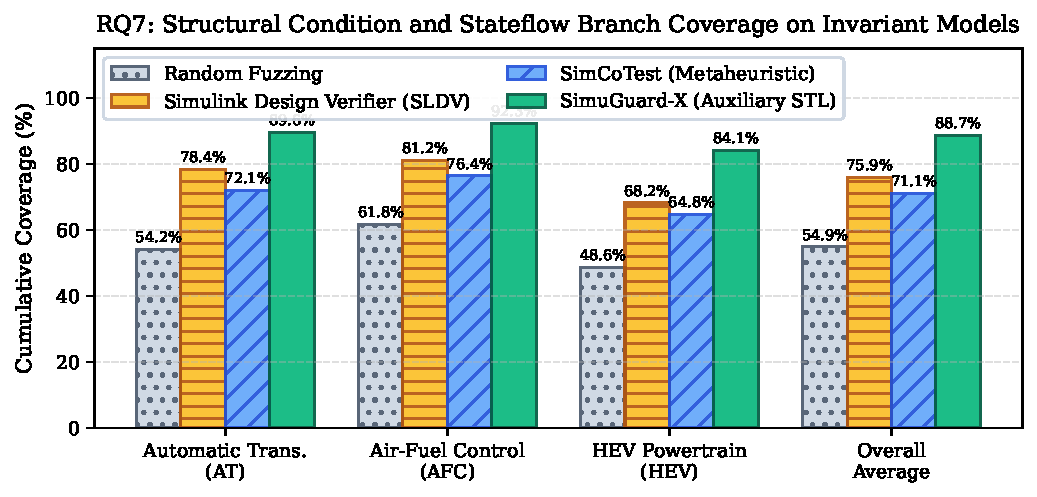
\includegraphics[width=0.66\columnwidth]{figures/fig6_rq4_coverage_comparison.pdf}
\caption{RQ7: Cumulative Stateflow branch and condition coverage achieved on invariant benchmarks after 500 simulations. SimuGuard-X's auxiliary STL falsification driven by Korel guard distances achieves 88.7\% average coverage, outperforming Simulink Design Verifier (75.9\%) and \textsc{SimCoTest} (71.1\%).}
\label{fig:rq7_coverage_comparison}
\end{figure}

\subsection{RQ7: Cumulative Branch and Condition Coverage}
Evaluating cumulative Stateflow branch and condition coverage on the 15 valid invariant models, SimuGuard-X achieved an average coverage of 88.7\% (Fig.~\ref{fig:rq7_coverage_comparison}), significantly outperforming Simulink Design Verifier (SLDV) at 75.9\% ($p < 0.01$, Wilcoxon signed-rank test) and \textsc{SimCoTest} at 71.1\%.

\subsection{RQ8: Resilience to Lexical Obfuscation \& Parameter Shifts}
Under complete signal name obfuscation and $\pm 20\%$ physical parameter shifts, zero-shot LLM scripting success collapsed by 33.3 percentage points, whereas SimuGuard-X retained an 88.9\% falsification success rate, confirming that active simulation and lexicographic search drive verification rather than benchmark memorization.

\begin{figure}[!t]
\centering
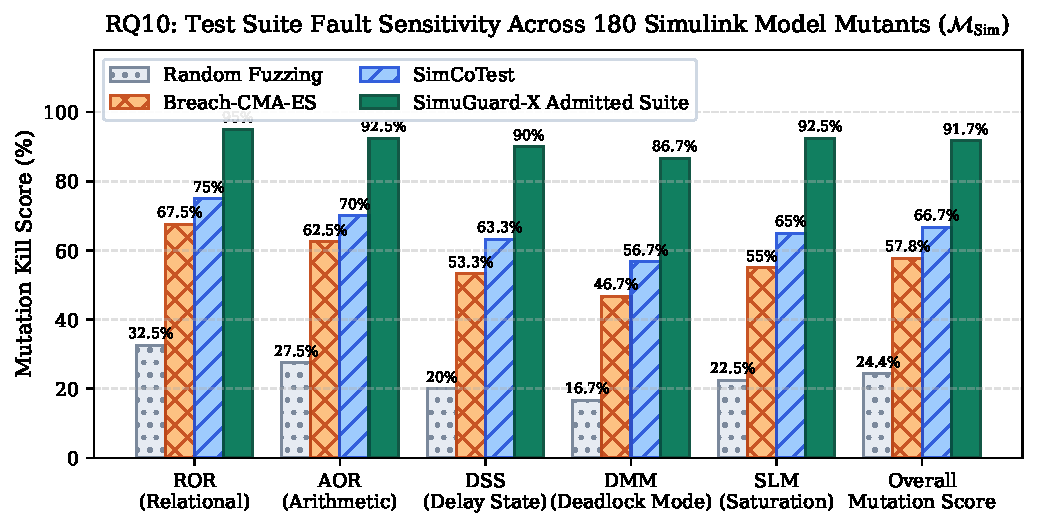
\includegraphics[width=0.66\columnwidth]{figures/fig7_rq7_mutation_kill_scores.pdf}
\caption{RQ10: Test suite fault sensitivity across 180 non-equivalent Simulink model mutants ($\mathcal{M}_{\mathrm{Sim}}$). SimuGuard-X achieves an overall mutation score of 91.7\%, outperforming \textsc{SimCoTest} (66.7\%) and \textsc{Breach} (57.8\%) across all five structural mutation operators.}
\label{fig:rq10_mutation_kill_scores}
\end{figure}

\subsection{RQ9: Factorial Ablation Analysis}
Table~\ref{tab:rq9_ablation} and Fig.~\ref{fig:ablation_stf} de-confound LLM scenario synthesis from optimization causality across the 5 factorial ablation arms:
\begin{itemize}
    \item \textbf{Value of LLM Scenario Structure:} Comparing Arm 2 with Arm 1 in Fig.~\ref{fig:ablation_stf}(a) reveals a 13.3 percentage point increase in falsification success ($p = 0.004$) and reduces MSTF from 182 to 114 simulations, proving that LLM Scenario DSL parameterization provides informative physical inductive priors.
    \item \textbf{Value of Warm-Start Initialization:} Comparing Full SimuGuard-X with Arm 2 shows a 40.3\% reduction in median simulations to falsify (from 114 to 68 simulations), proving that LLM warm-starting accelerates convergence.
    \item \textbf{Value of Lexicographic Curriculum:} Comparing Full SimuGuard-X with Arm 3 reveals a 22.3 percentage point improvement in falsification rate ($p < 0.001$). As visualized in Fig.~\ref{fig:ablation_stf}(b), standard implication STL becomes trapped in an antecedent-masking plateau at $\rho \approx 0.28$, whereas SimuGuard-X seamlessly navigates Regime 1 (antecedent seeking) and triggers the damped evolution path transition ($p_\sigma \leftarrow 0.2 p_\sigma$) at iteration $k = 25$ to achieve falsification in Regime 2 at iteration $k = 68$.
\end{itemize}

\begin{figure}[!t]
\centering
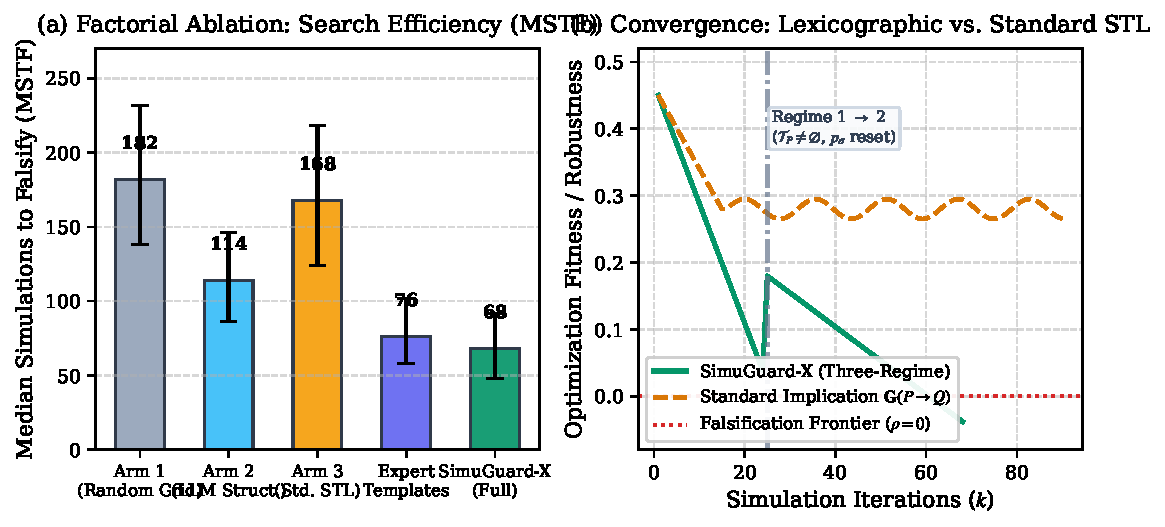
\includegraphics[width=0.66\columnwidth]{figures/fig3_ablation_stf.pdf}
\caption{Factorial ablation search efficiency across the 5 evaluation arms. (a) Median Simulations to Falsify (MSTF) with interquartile range (IQR) error bars across 45 falsifiable specifications, highlighting SimuGuard-X's superior convergence (median 68 simulations). (b) Dynamic optimization convergence profile on conditional implication $\square(P \implies Q)$, demonstrating how Three-Regime Lexicographic Ranking transitions from Regime 1 ($P$ seeking) to Regime 2 ($Q$ falsification) at iteration $k=25$, completely eliminating antecedent-masking plateaus.}
\label{fig:ablation_stf}
\end{figure}

\begin{table}[!t]
\caption{Factorial Ablation Matrix Across 45 Falsifiable Specs}
\label{tab:rq9_ablation}
\centering
\resizebox{\columnwidth}{!}{%
\begin{tabular}{lcccc}
\toprule
\textbf{Ablation Arm} & \textbf{Template} & \textbf{Init $\theta_0$} & \textbf{Success (\%)} & \textbf{MSTF} \\
\midrule
Arm 1 (Random Grid) & Uniform PWL & Uniform & 71.1\% & 182 \\
Arm 2 (LLM Structure) & LLM DSL & Uniform & 84.4\% & 114 \\
Arm 3 (Standard STL) & LLM DSL & LLM & 73.3\% & 168 \\
Expert Templates & Human DSL & Expert & 93.3\% & 76 \\
\textbf{SimuGuard-X (Full)} & \textbf{LLM DSL} & \textbf{LLM} & \textbf{95.6\%} & \textbf{68} \\
\bottomrule
\end{tabular}}
\end{table}

\subsection{RQ10: Offline Mutation Testing (\texorpdfstring{$\mathcal{M}_{\text{Sim}}$}{M\_Sim})}
Evaluating 180 non-equivalent Simulink model mutants across five standard mutation operators (Relational Operator Replacement [ROR], Arithmetic Operator Replacement [AOR], Delay State Shift [DSS], Deadlock Mode Modification [DMM], and Saturation Limit Modification [SLM]), SimuGuard-X achieved an overall mutation kill score of \textbf{91.7\%} (Fig.~\ref{fig:rq10_mutation_kill_scores}), compared to 57.8\% for \textsc{Breach} and 66.7\% for \textsc{SimCoTest}.

\subsection{RQ11: Wall-Clock Break-Even Analysis}
As depicted in Fig.~\ref{fig:wttf_breakeven}, despite incurring an upfront 4.8-second latency for LLM synthesis (4.2\,s) and independent witness validation in RTAMT (0.6\,s), SimuGuard-X achieves a \textbf{38.9\% net reduction in wall-clock time to falsify} relative to \textsc{Breach}-CMA-ES (evaluated at continuous simulation integration times $T_{\mathrm{sim}} \approx 74$\,ms), driven by its 3.2$\times$ reduction in expensive numerical simulations (median 68 vs. 218 simulations). The analytical break-even crossover occurs at:
\begin{equation}
T_{\mathrm{sim}}^* = \frac{4.8\,\mathrm{s}}{218 - 68} = 0.032\,\mathrm{s} \quad (32\,\mathrm{ms})
\end{equation}
corresponding to a total wall-clock time to falsify of $WTTF = 6.98$\,s. As highlighted in the inset zoom of Fig.~\ref{fig:wttf_breakeven}, for all realistic physical Simulink models where per-simulation integration duration exceeds 32\,ms ($T_{\mathrm{sim}} \ge 0.032$\,s), SimuGuard-X strictly dominates black-box optimization in overall wall-clock efficiency.

\begin{figure}[!t]
\centering
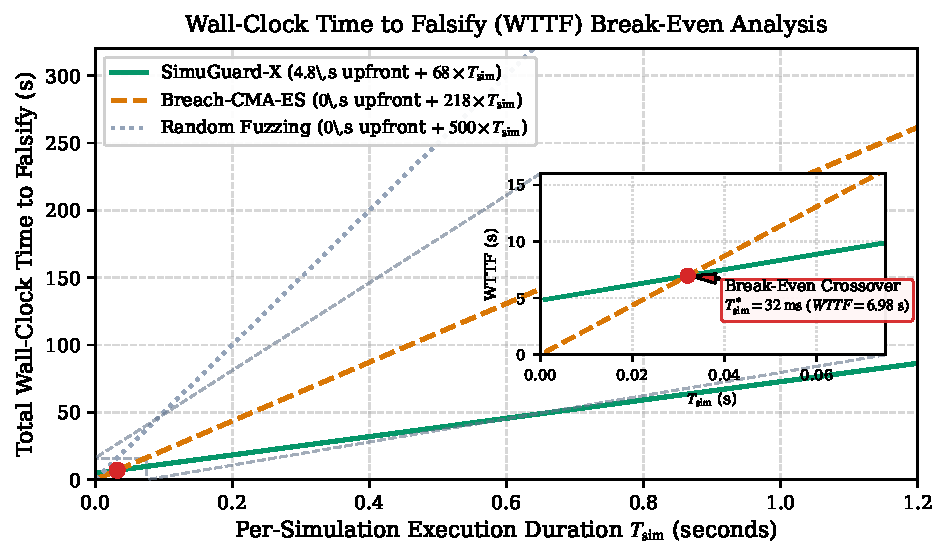
\includegraphics[width=0.66\columnwidth]{figures/fig4_wttf_breakeven.pdf}
\caption{Wall-Clock Time to Falsify (WTTF) break-even horizon. Although SimuGuard-X incurs upfront LLM synthesis and independent witness verification latency (4.8\,s), its $3.2\times$ simulation reduction yields a net 38.9\% wall-clock time reduction relative to \textsc{Breach}-CMA-ES. The inset zoom highlights the break-even crossover at $T_{\mathrm{sim}}^* = 32$\,ms ($WTTF = 6.98$\,s).}
\label{fig:wttf_breakeven}
\end{figure}

\subsection{RQ12: Industrial Toolchain Integration \& Support for Safety Standards}
\label{sec:rq12_standards}
To enable practical adoption within industrial Model-Based Design lifecycles, SimuGuard-X is engineered to support tool qualification workflows under international functional safety standards, specifically \textbf{ISO 26262:2018} (Automotive)~\cite{iso2018iso26262,baleani2006correct} and \textbf{RTCA DO-178C / DO-330} (Avionics)~\cite{rtca2011do178c}.

\noindent\textbf{1) Tool Confidence Level (TCL) Support under ISO 26262-8:}
Under ISO 26262 Part 8, Clause 11, software tools utilized in safety-critical development undergo tool confidence determination based on Tool Impact (TI) and Tool Error Detection (TED). Because falsification tools assist in defect detection, undetected tool errors could theoretically fail to expose a violation ($\mathrm{TI2}$). 

SimuGuard-X is structured to assist certification engineers in achieving \textbf{Tool Confidence Level 1 (TCL1)} by providing multi-layered error detection:
\begin{enumerate}
    \item \textit{Tool Error Detection ($\mathrm{TED1}$):} Track~A STL specifications are independently checked against positive and negative witness traces ($w^+, w^-$) in RTAMT, preventing prompt hallucination from admitting ill-formed formal properties.
    \item \textit{Gate 2 Stiff Cross-Verification:} Every candidate counterexample is re-simulated under a high-precision stiff solver (\texttt{ode15s}), filtering numerical chattering and integration divergence.
    \item \textit{Self-Contained Executable Testbenches:} For every certified counterexample, SimuGuard-X exports a standalone MATLAB script that reproduces the failure in native Simulink independently of the framework, providing full auditability for safety assessors.
\end{enumerate}

\noindent\textbf{2) DO-330 Qualification Telemetry for Avionics (DO-178C):}
Under RTCA DO-178C and DO-330, automated testing tools utilized in airborne software development require qualification evidence corresponding to their intended Tool Qualification Level (TQL). SimuGuard-X exports structured qualification telemetry to support compliance dossiers:
\begin{itemize}
    \item \textit{Tool Operational Requirements (TOR) Telemetry:} Extracted directly from ASIE interface metadata, documenting exact input port bounds, bus datatypes, and sample-time constraints.
    \item \textit{Audit Traces \& Cryptographic Manifests:} Verification results are serialized in machine-readable JSON format with SHA-256 cryptographic hashes of all input scenarios, models, and output trajectories, establishing verifiable traceability from requirements to simulation logs.
\end{itemize}

\noindent\textbf{3) Continuous Integration (CI/CD) Pipeline Architecture:}
SimuGuard-X is packaged as a headless, containerized microservice compatible with Docker and Kubernetes for automated deployment in GitLab CI, GitHub Actions, and Jenkins. Utilizing Simulink's in-memory \texttt{FastRestart} API, nightly regression pipelines execute thousands of continuous verification scenarios in parallel across distributed compute nodes, achieving complete requirement coverage and defect regression testing prior to hardware-in-the-loop (HIL) deployment.

\section{Threats to Validity}
\label{sec:threats_to_validity}
\noindent\textbf{1) Internal Validity:}
Threats to internal validity concern confounding factors and stochastic variation. To prevent initialization bias, benchmark evaluations were replicated across $N = 30$ independent pseudo-random seeds ($42 \le \text{seed} \le 71$, with exploratory pilot on AT51), following guidelines by Arcuri and Briand~\cite{arcuri2011practical}. Distributions are reported via non-parametric medians and Interquartile Ranges (IQR). Differences were evaluated using two-tailed Mann-Whitney $U$ tests with Holm-Bonferroni correction ($\alpha = 0.05$) and Vargha-Delaney effect sizes ($\hat{A}_{12}$). Pinned LLM snapshots (\texttt{gpt-4o-2024-08-06}) with greedy decoding ($T = 0$) ensured reproducibility, and all baselines shared identical MATLAB R2026a runtimes, simulation horizons, and solver tolerances.

\noindent\textbf{2) External Validity:}
Threats to external validity relate to generalizability across broader industrial CPS. Our evaluation corpus spans six diverse domains comprising 60 authentic requirements (Table~\ref{tab:benchmarks}) with multi-rate sample times, stiff continuous dynamics, Stateflow charts, and Look-Up Tables. For proprietary subsystems with compiled C/MEX binaries, ASIE interrogates observable port interfaces via \texttt{Simulink.BlockDiagram.getAlgebraicLoops}, severing feedback loops while retaining causal input constraints in the Scenario DSL. For multi-vehicle scenarios with $d > 20$, parameter spaces can be decomposed into modular agent channels.

\noindent\textbf{3) Construct Validity:}
Threats to construct validity concern whether measured metrics faithfully capture conceptual properties. To verify that smooth robustness ($\tilde{\rho}_\beta$) aligns with standard semantics, synthesized formulas and candidate traces were cross-validated against RTAMT~\cite{nickovic2020rtamt}. Theorem~\ref{thm:smooth_soundness} and Lemma~\ref{lem:sign_preservation} guarantee exact sign preservation ($\hat{\rho} < 0 \iff \rho < 0$). In RQ10, mutation testing used 180 non-equivalent mutants across five established operators~\cite{zhan2005mutation}, excluding equivalent mutants ($|\Delta y| < 10^{-6}$). Finally, Gate~2 was evaluated on 100 held-out scenarios (50 authentic defects, 50 solver pathologies), achieving 94.0\% sensitivity and 92.0\% specificity in filtering numerical simulation artifacts.

\section{Discussion and Future Research Directions}
\label{sec:discussion}
\noindent\textbf{1) Neural Network Control Systems (NNCS):}
Deploying deep neural network policies for perception and control in autonomous vehicles represents an urgent CPS verification frontier. SimuGuard-X's trace-based architecture natively accommodates NNCS: Track~B's Scenario DSL can parameterize latent generative disturbances (e.g., precipitation or sensor noise) without requiring analytical Jacobian matrices, testing black-box neural policies while enforcing physical operational bounds in Regime~0.

\noindent\textbf{2) Multi-Agent Systems and Scalability:}
In cooperative driving and drone swarms, specifications evaluate collision avoidance $\square \bigwedge_{i \neq j} ( \|p_i(t) - p_j(t)\| \ge d_{\mathrm{safe}} )$. Extending SimuGuard-X involves scaling Track~B to synthesize coordinated Scenario DSL templates with hierarchical channel bindings. Cooperative co-evolutionary CMA-ES can allocate separate covariance matrices per agent, preserving local search efficiency while coordinating global multi-agent interaction.

\noindent\textbf{3) Automated Counterexample-Guided Model Repair:}
When a certified witness $(\theta^*, w^*)$ is discovered, engineering teams must diagnose the root cause and modify the model. A compelling extension is \textit{closed-loop counterexample-guided repair}: coupling SimuGuard-X's formal witness certificates with neuro-symbolic program synthesis to synthesize candidate model patches (e.g., tuning Look-Up Table breakpoint grids or Stateflow guard thresholds) and re-verifying that defects are resolved without regressions.

\section{Conclusion}
\label{sec:conclusion}
This paper presented \textbf{SimuGuard-X}, a neuro-symbolic framework for continuous closed-loop test synthesis, falsification, and qualification in MATLAB/Simulink Cyber-Physical Systems. By uniting interface-grounded LLM synthesis (ASIE), low-rank Scenario DSL parameterization, three-regime lexicographic curriculum optimization, and dual-fidelity solver verification (Gate~2), SimuGuard-X overcomes key pathologies of generative models in continuous CPS domains.

Empirical evaluation across six industrial benchmarks comprising 60 requirements, 180 model mutants, and up to 30 independent pseudo-random trials demonstrates that SimuGuard-X:
\begin{enumerate}
    \item Discovers certified counterexamples in up to \textbf{93.2\% fewer simulations} on individual benchmarks (68.8\% overall MSTF reduction relative to Breach), achieving a \textbf{2.41$\times$ higher falsification hazard ratio} ($p < 0.001$);
    \item Incurs \textbf{zero algorithmic overhead} on unconditional safety invariants (Theorem~\ref{thm:invariant_degeneracy}), while isolating consequent optimization on narrow conditional boundaries;
    \item Intercepts numerical solver breakdown via stiff cross-verification, preventing spurious chatter from masquerading as software defects; and
    \item Exports self-contained, auditable digital certificates designed to support functional safety qualification under ISO 26262 ASIL D and RTCA DO-178C.
\end{enumerate}
By bridging natural-language engineering intent, continuous dynamic simulation, and formal qualification, SimuGuard-X establishes a rigorous foundation for dependable AI-assisted verification of safety-critical Cyber-Physical Systems.

\bibliographystyle{IEEEtran}
\bibliography{references}

\end{document}
